%%%%%%%%%%%%%%%%%%%%%%%%%%%%%%%%%%%%%%%%%%%%%%%%%%%%%%%%%%
%%
%%  LOD-L9.tex
%%  Lecture 9: Modeling: Manifolds, Orbifolds and Quasifolds
%%
%%%%%%%%%%%%%%%%%%%%%%%%%%%%%%%%%%%%%%%%%%%%%%%%%%%%%%%%%%

\chapter*{\S L9. Modeling: Manifolds, Orbifolds and Quasifolds}
\setcounter{footnote}{0}

%%%%%%%%%%%%%%%%%%%%%%%%%%%%%%%%%%%%%%%%%%%%%%%%%%%%%%%%%%
%%
%% MARK: Abstract
%%
%%%%%%%%%%%%%%%%%%%%%%%%%%%%%%%%%%%%%%%%%%%%%%%%%%%%%%%%%%
\begin{abstract}
  In this lecture we build the category of orbifolds,
  and also quasifolds,
  by modeling locally these spaces according to what they should look like;
  and manifolds, of course.
\end{abstract}

%%%%%%%%%%%%%%%%%%%%%%%%%%%%%%%%%%%%%%%%%%%%%%%%%%%%%%%%%%
%%
%% MARK: Introduction
%%
%%%%%%%%%%%%%%%%%%%%%%%%%%%%%%%%%%%%%%%%%%%%%%%%%%%%%%%%%%

Orbifolds have been introduced by Ishiro Satake as \emph{V-Manifolds} in 1956 and 1957 \cite{Sat56} \cite{Sat57}.
They have been presented as smooth structures for describing quotient spaces by a finite group of transformations.
We shall recall Satake's construction first and show then how we can rethink these spaces as diffeological spaces.

We show in particular how diffeology solves,
in a pure geometrical way,
a problem unresolved by Satake and successors,
about what are smooth maps between orbifolds,
and build then the subcategory \{Orbifolds\} in the category \{Diffeology\}.
\begin{figure}[ht]
  \centerline{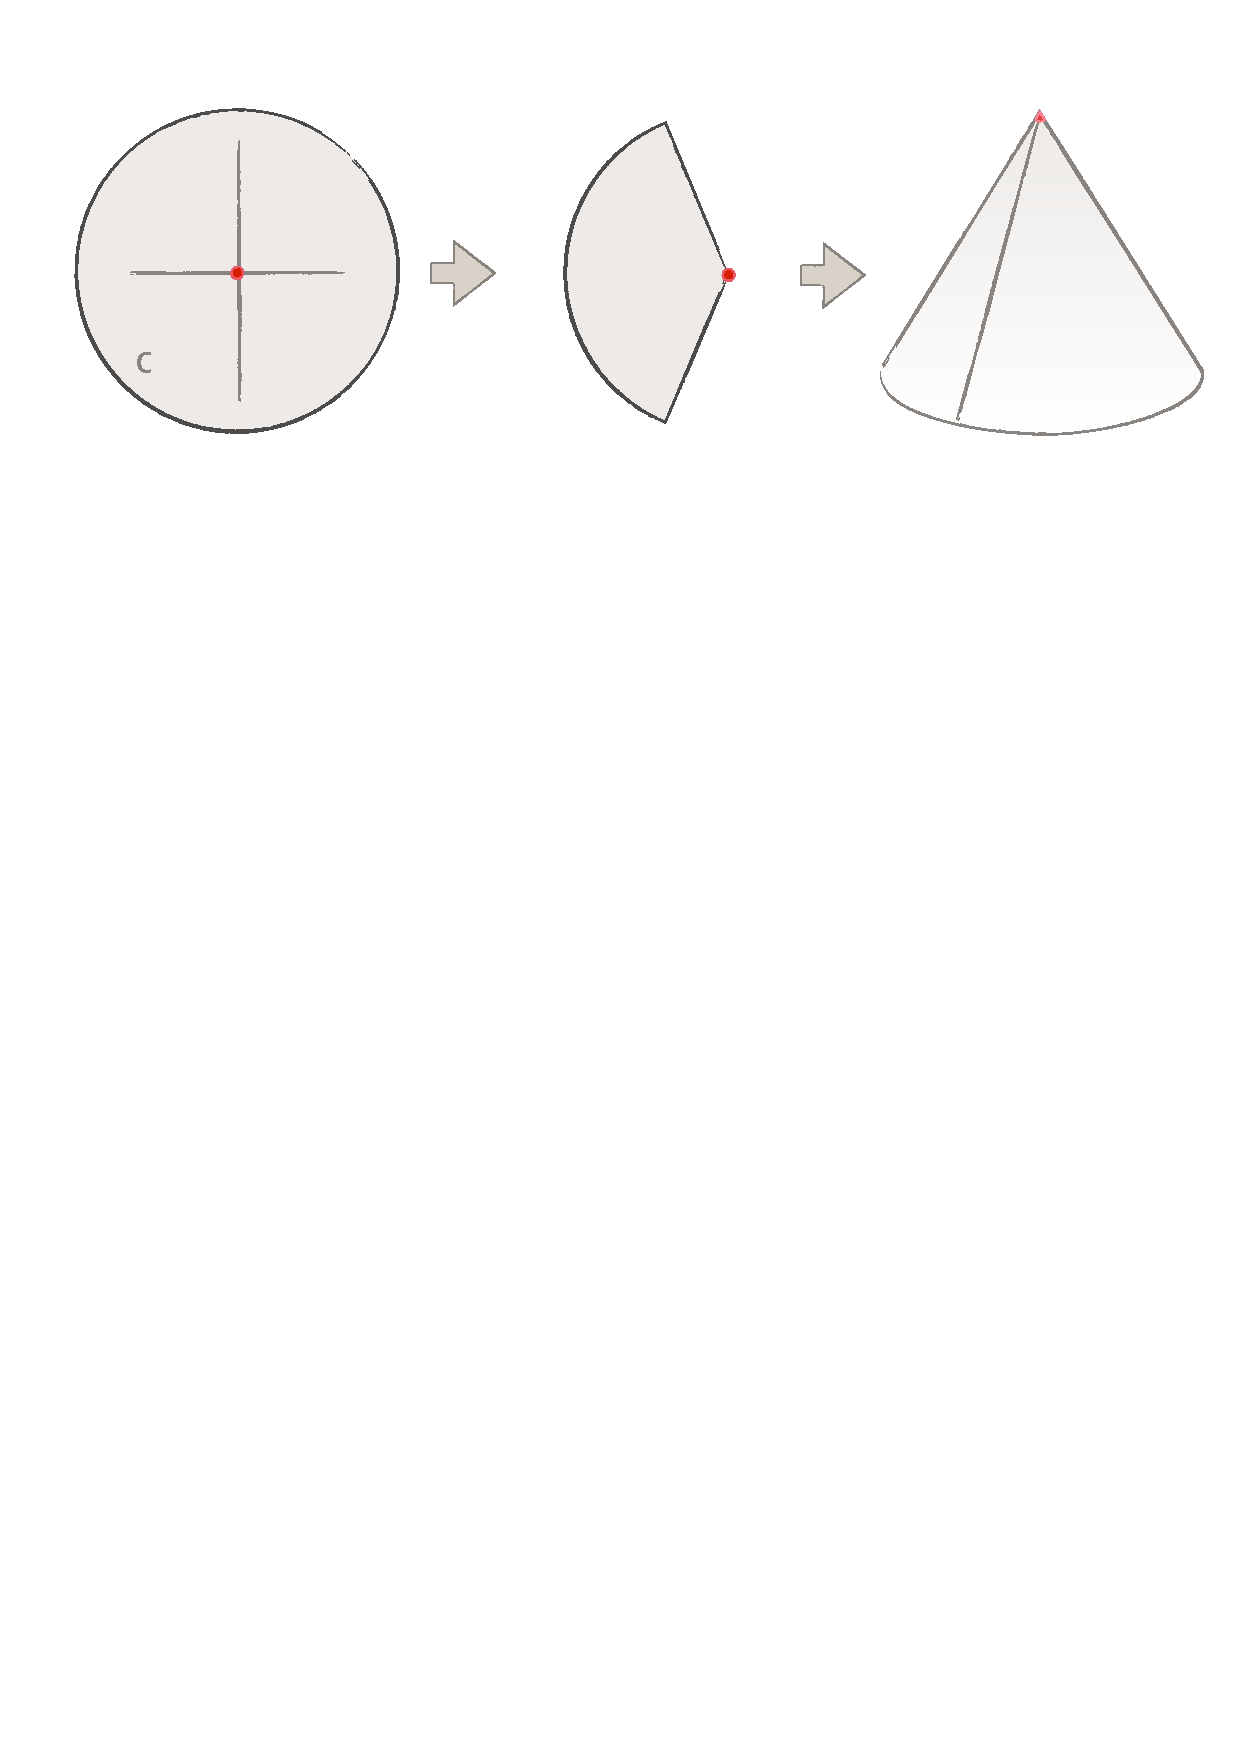
\includegraphics[width=\textwidth]{Figures/Cone.pdf}}
  \caption{\small The cone orbifold viewed by a topologist.}
  \label{fig-cone}
\end{figure}

Let us mention that the word \emph{orbifold} has been coined by Thurston \cite{Thu78} in 1978 as a substitute for \emph{V-manifold},
but it recovers the same original Satake notion without modification.
This concept was introduced to describe the smooth structure of spaces that look like manifolds,
except on a few points or subsets,
where they look like quotients of linear domains by a finite group of linear transformations.

The typical example is the quotient of the field $\CC$ by a group of roots of unity.%
\footnote{We consider $\CC$ for its field structure: addition and multiplication,
not for its complex structure which is anecdotal here.}
The quotient space is always drawn as a cone as shown by Figure \ref{fig-cone},
to suggest the singularity of the point $0$.
But how do we capture the smooth structure around the singular point?
\uline{That is the whole question}.

%%%%%%%%%%%%%%%%%%%%%%%%%%%%%%%%%%%%%%%%%%%%%%%%%%%%%%%%%%
%%
%% MARK:  Orbifolds, the Satake Definition
%%
%%%%%%%%%%%%%%%%%%%%%%%%%%%%%%%%%%%%%%%%%%%%%%%%%%%%%%%%%%
\section{Orbifolds, the Satake definition}

The elementary brick in Satake's construction is the Local Uniformization System.
It is a topological construction.

%%###########
% MARK: Figure
%%###########
\begin{figure}[htb]
  \centerline{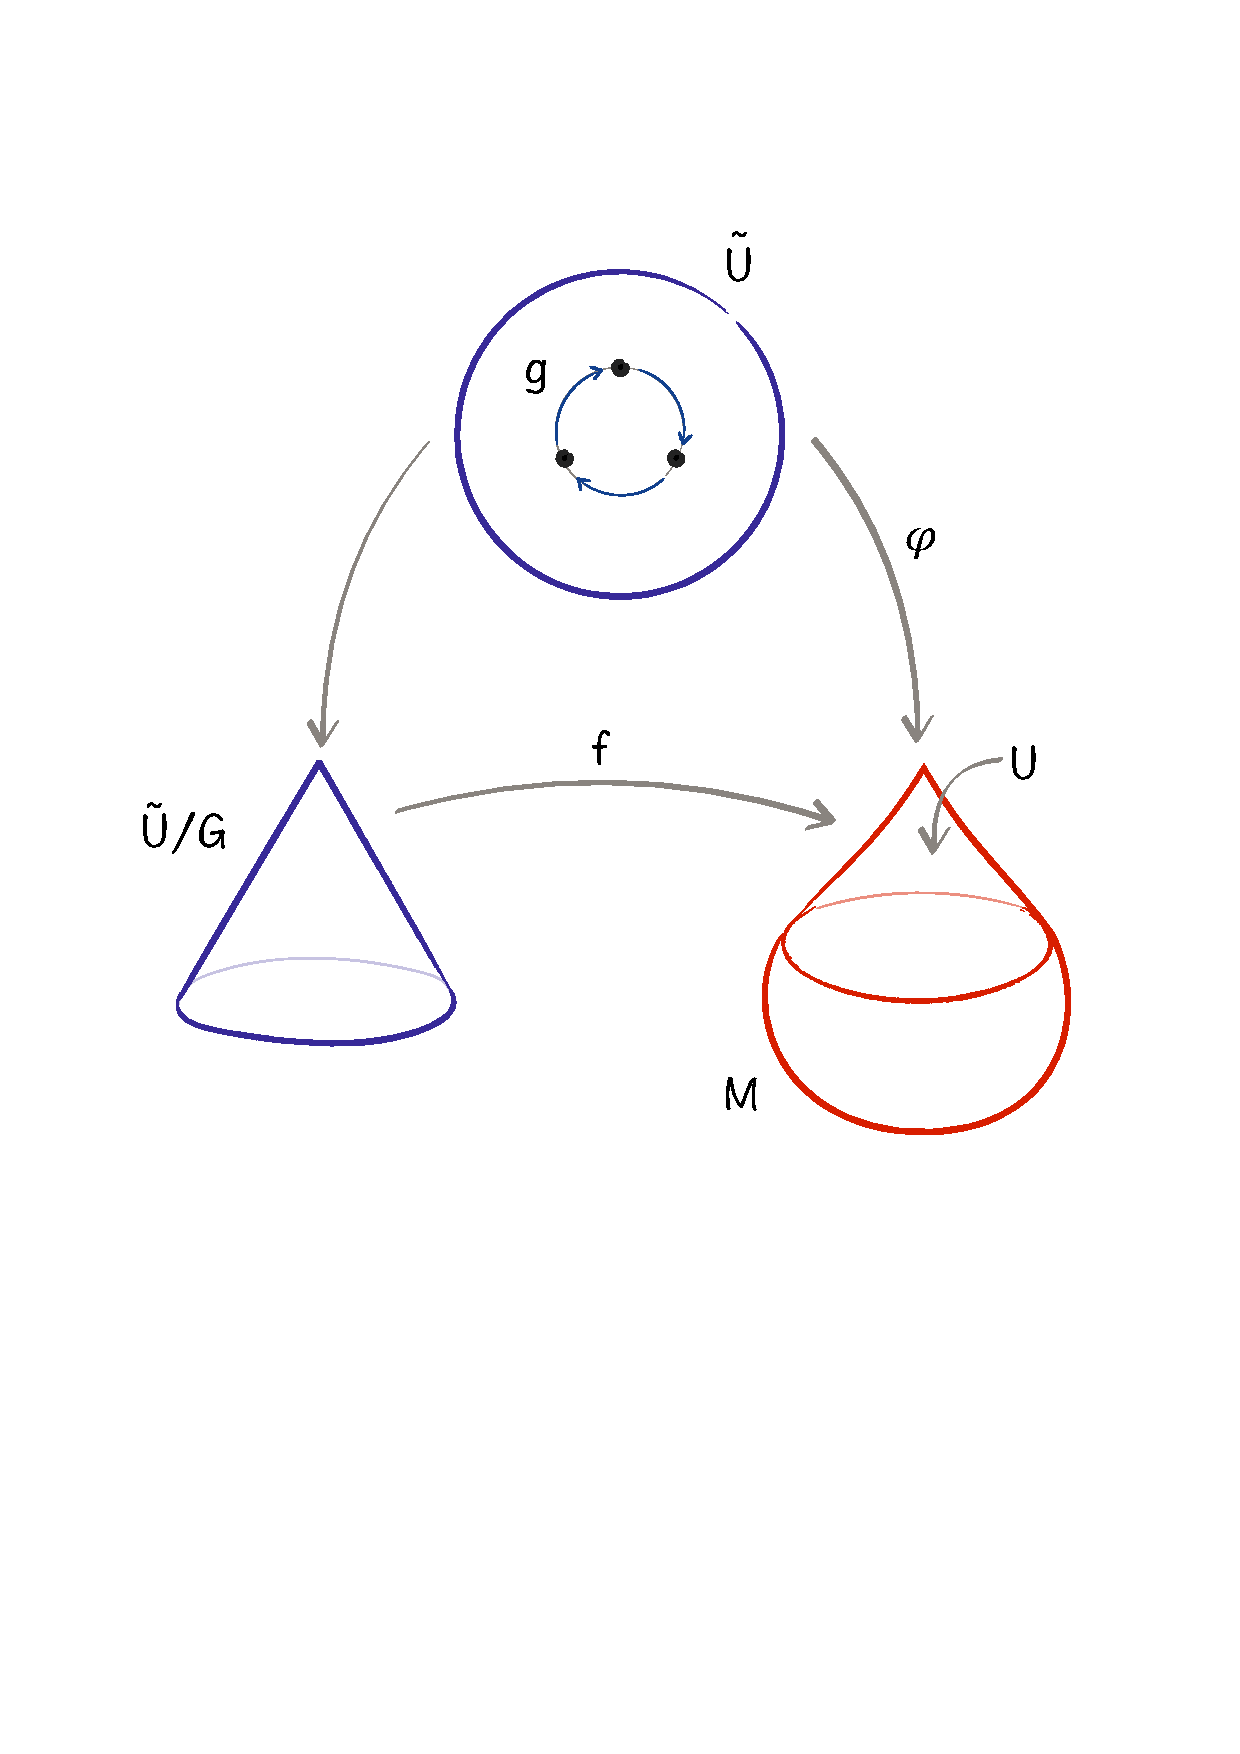
\includegraphics[width=.50\textwidth]{Figures/fig-lus.pdf}}
  \caption{Local Uniformizing System.}
  \label{lus}
\end{figure}
%%###########

\begin{Article}{Local uniformization system.}{}
  Let $M$ be a Hausdorff space and $U \subset M$ an open subset.
  A \emph{local uniformizing system for $U$} (l.u.s) is a triple $(\tilde{U}, G, \varphi)$,
  where $\tilde{U}$ is a connected open subset of $\RR^n$ for some $n$,
  where $G$ is a finite group of diffeomorphisms of $\tilde{U}$,%
  \footnote{in the original definition,
  the fixed point sets have codimension $\geq 2$.}
  and where $\varphi \colon \tilde{U} \to U$
  is a map which induces a homeomorphism between $\tilde{U}/G$ and $U$.

  \uline{Note.} In Figure \ref{lus},
  $f$ is this homeomorphism from $\tilde U/G$ to $U$.
\end{Article}

Local uniformizing systems are patched together by {\itshape injections};
these can be thought of as the ``\uline{transition maps}''.
The following definition is taken from \cite[p.~466]{Sat57}:

\begin{Article}{Injections.}{}
  \label{art-injection}
  An \emph{injection} from an l.u.s $(\tilde{U}, G, \varphi)$ to another l.u.s $(\tilde{U'}, G', \varphi')$ is a diffeomorphism $\lambda$ from $\tilde{U}$ onto an open subset of $\tilde{U'}$ such that
  $$
    \varphi = \varphi' \circ \lambda.
  $$
\end{Article}

%%###########
% MARK: Figure
%%###########
\begin{figure}[htb]
  \centerline{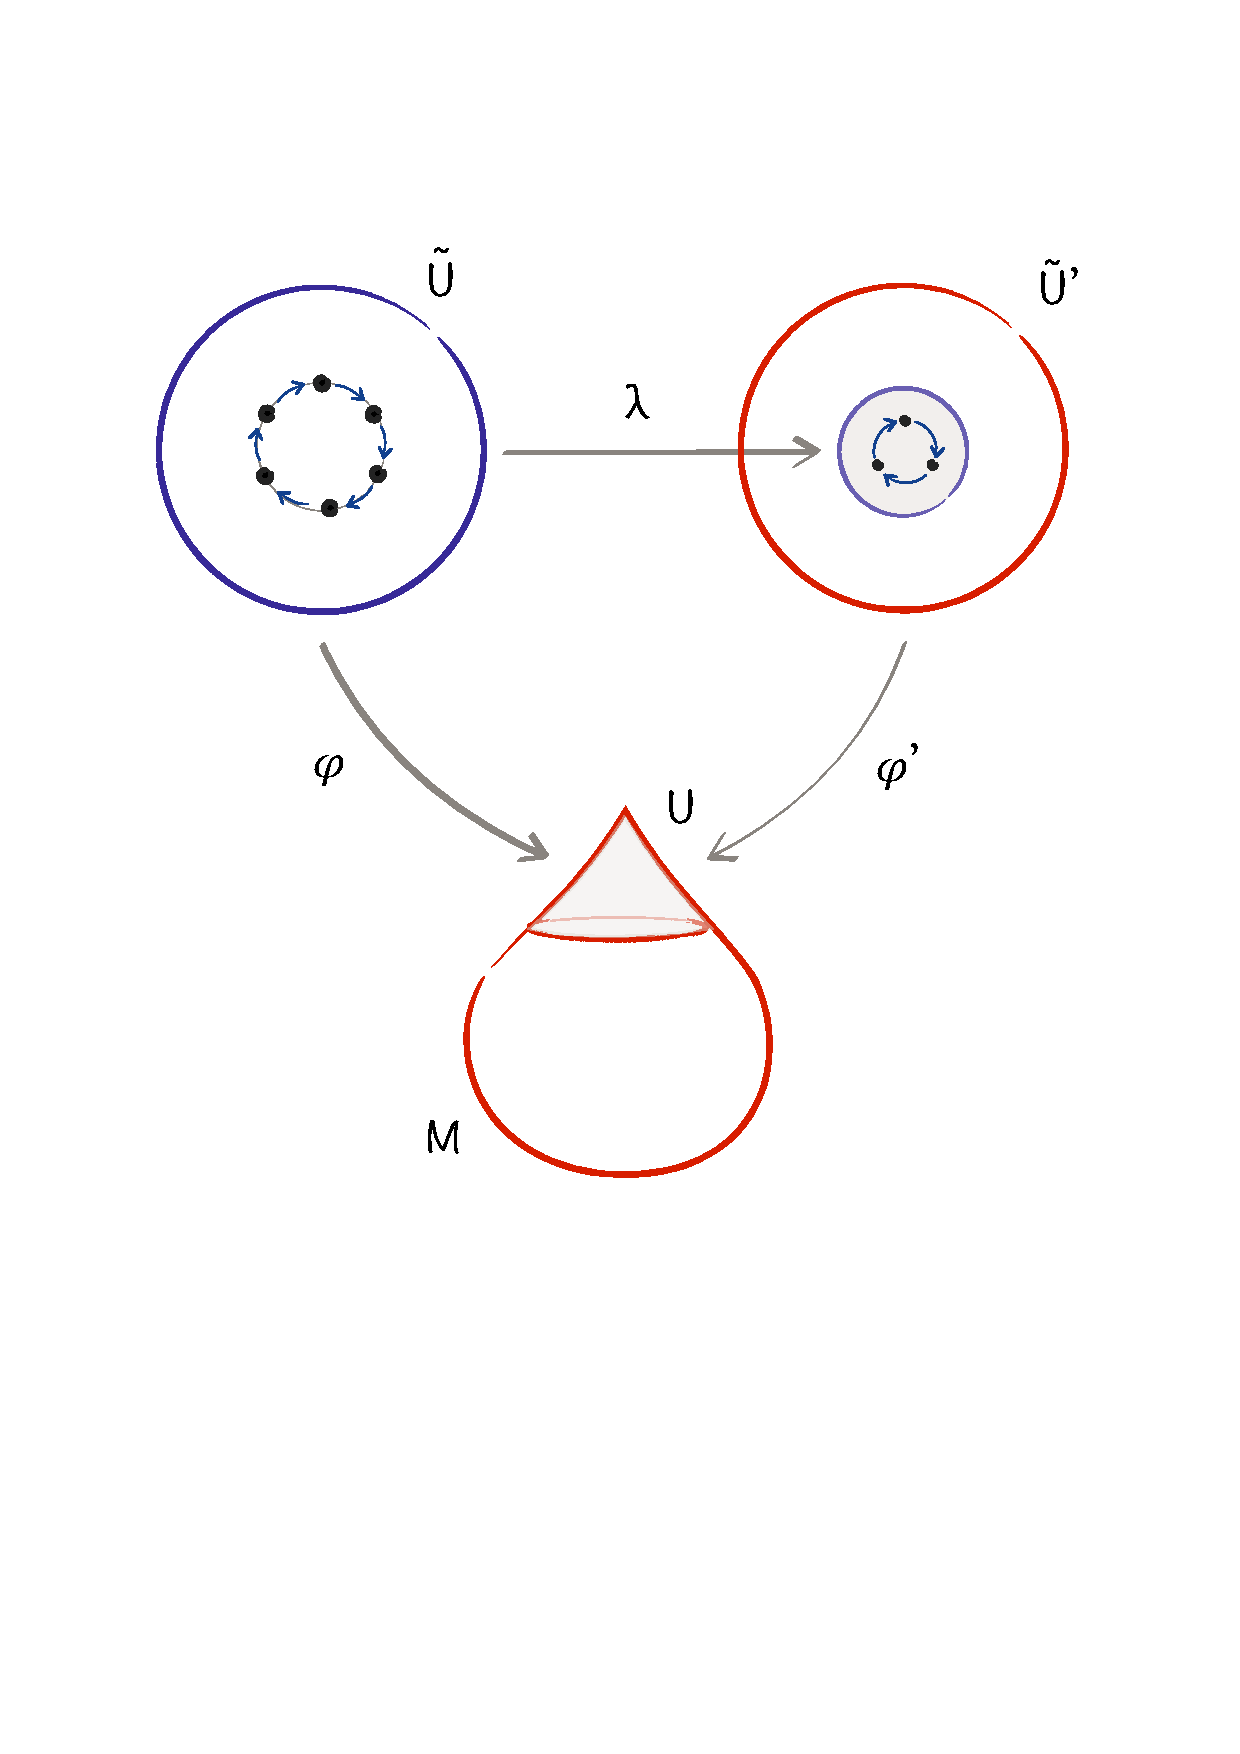
\includegraphics[width=.50\textwidth]{Figures/fig-injection.pdf}}
  \caption{Injection.}
  \label{injection}
\end{figure}
%%###########

\begin{Article}{Defining family.}{}
  \label{art-defining-family}
  Let $M$ be a Hausdorff space.
  A \emph{defining family} on $M$ is a family $\cF$ of l.u.s for open subsets of $M$,
  satisfying conditions below.
  An open subset $U \subset M$ is said to be $\cF$-\emph{uniformized} if there exists an l.u.s. $(\tilde{U},G,\varphi)$ in $\cF$ such that $\varphi(\tilde{U}) = U$.
  \begin{enumerate}
    \item
    Every point in $M$ is contained in one $\cF$-uniformized open set,
    at least.
    If a point $p$ is contained in two $\cF$-uniformized open sets $U_1$ and $U_2$,
    then there exists an $\cF$-uniformized open set $U_3$ such that $p \in U_3 \subset U_1 \cap U_2$.
    \item
    If $(\tilde{U},G,\varphi)$ and $(\tilde{U'},G',\varphi')$ are l.u.s in $\cF$ and $\varphi(\tilde{U}) \subset \varphi'(\tilde{U'})$,
    then there exists an injection $\lambda \colon \tilde{U} \to \tilde{U'}$.
  \end{enumerate}
  %
  In other words,
  if $p \in U \cap U'$ there exists a third l.u.s. $(\tilde{U''},G'',\varphi'')$,
  two injections $\lambda \colon \tilde U'' \to \tilde U$ and $\lambda' \colon \tilde U'' \to \tilde U'$ such that $\pphi' \circ \lambda' = \pphi'' = \pphi \circ \lambda$,
  as shown in Figure \ref{fig-defining-family}.
\end{Article}

%%###########
% MARK: Figure
%%###########
\begin{figure}[htb]
  \centerline{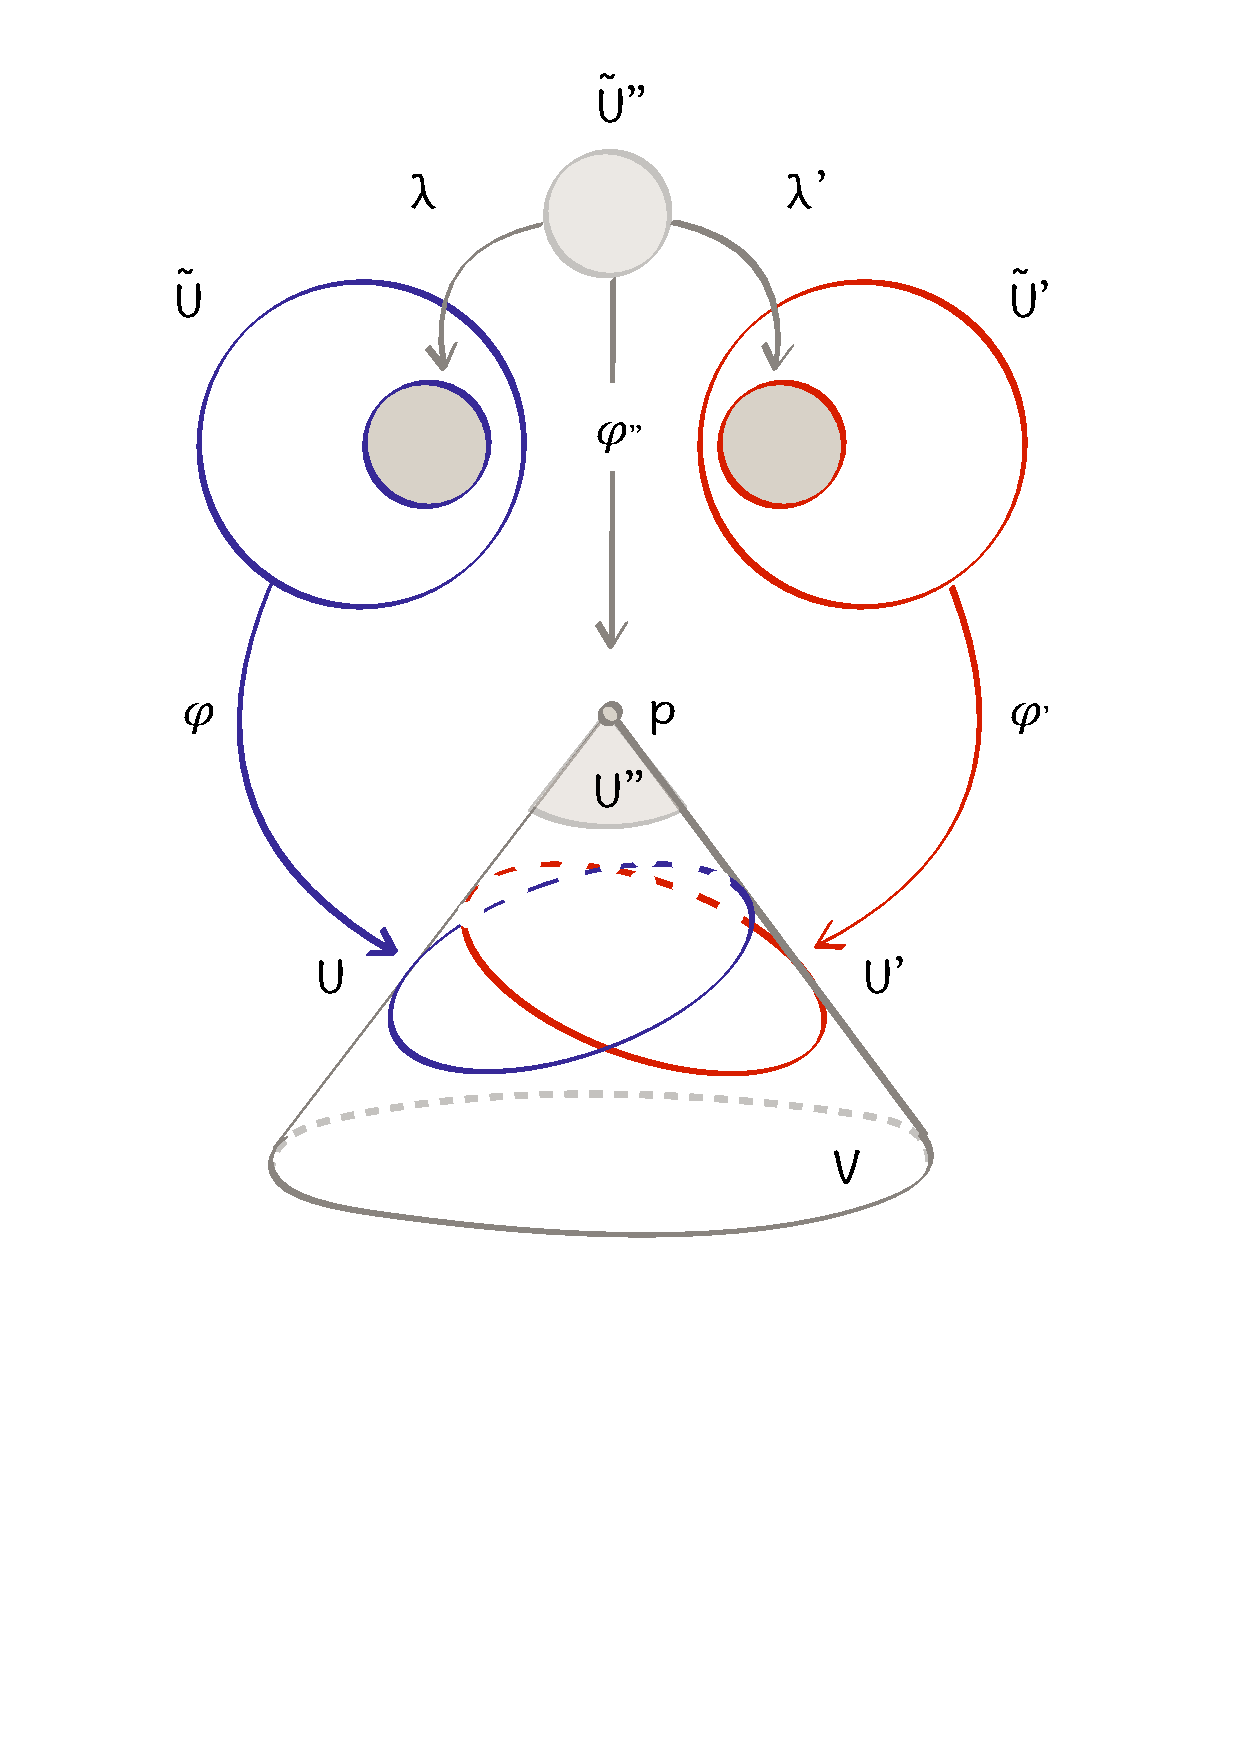
\includegraphics[width=.50\textwidth]{Figures/fig-defining-family.pdf}}
  \caption{Defining Family.}
  \label{fig-defining-family}
\end{figure}
%%###########

\begin{Article}{V-manifold.}{}
  \label{V-Manifold}
  The following definition is taken from \cite[p.~467, Definition 1]{Sat57}.

  \uline{Definition.}~{\itshape A \emph{V-manifold} is a composite concept formed of a Hausdorff topological space $M$ and a defining family $\cF$.}

  Two defining families $\cF$ and $\cF'$ are said to be \emph{directly equivalent} if there exists a third defining family $\cF''$ containing both of them.
  Two defining families are said to be \emph{equivalent} if they are the ends of a chain of directly equivalent defining families.
  Equivalent families are regarded as defining one and the same V-manifold structure on $M$.

  In \cite[p.~467, footnote 1]{Sat57} Satake writes:
  \begin{quote}
    \emph{But in the following we consider a V-manifold $M$ with a fixed defining family $\cF$.
    (i.e. a ``\emph{coordinate V-manifold}'' $(M, \cF)$.}
  \end{quote}

  That is the convention we have made and when we say {\em V-manifold} it is always a coordinate V-manifold $(M, \cF)$ we have in mind.
\end{Article}

%%%%%%%%%%%%%%%%%%%%%%%%%%%%%%%%%%%%%%%%%%%%%%%%%%%%%%%%%%
%%
%% MARK:  Orbifolds as Diffeologies
%%
%%%%%%%%%%%%%%%%%%%%%%%%%%%%%%%%%%%%%%%%%%%%%%%%%%%%%%%%%%
\section{Orbifolds as diffeologies}

\begin{Article}{Diffeological orbifolds.}{}
  \label{Diffeological-Orbifolds}
  Let $X$ be a diffeological space.
  We say that $X$ is a \emph{diffeological $n$-orbifold} (or a D-orbifold) if $X$ is everywhere locally diffeomorphic to some $\RR^n/\Gamma$,
  with $\Gamma$ a finite subgroup of $\GL(n,\RR)$,
  possibly different from point to point.
  The diffeological $n$-orbifolds are modeled on quotient spaces of type $\RR^n/\Gamma$.

  More precisely,
  for every point $x \in X$,
  there exists a finite group $\Gamma \subset \GL(n,\RR)$,
  a (connected) $\Gamma$-invariant Euclidean domain $\tilde U \subset \RR^n$ and a local diffeomorphism $F : \tilde U/\Gamma \to X$ on a neighborhood of $x$.

  The situation,
  illustrated in Figure \ref{D-orbifold},
  looks like the previous definition of l.u.s except that here the quotient $\tilde U/\Gamma$ is equipped with the quotient diffeology,
  the map $\Class \colon \RR^n \to \RR^n/\Gamma$ is the canonical subduction and $F$ is a local diffeomorphism.

  These local diffeomorphisms are called \emph{charts} of the D-orbifold $X$.
  An atlas of $X$ is any covering set $\cA$ of charts.
  Of course there exists a \emph{saturated atlas} made of all charts.

  Given an atlas $\cA$ of $X$,
  that defines a generating family
  $$
    \cF = \{ F \circ \Class \mid F \in \cA\},
  $$
  where $\Class$ is relative to the group $\Gamma$ associated with $F$.
  We call $\cF$ the \emph{strict generating family} associated with the atlas $\cA$.

  Note that when $\Gamma$ is trivial we get the classical manifolds.
\end{Article}

%%###########
% MARK: Figure
%%###########
\begin{figure}[htb]
  \centerline{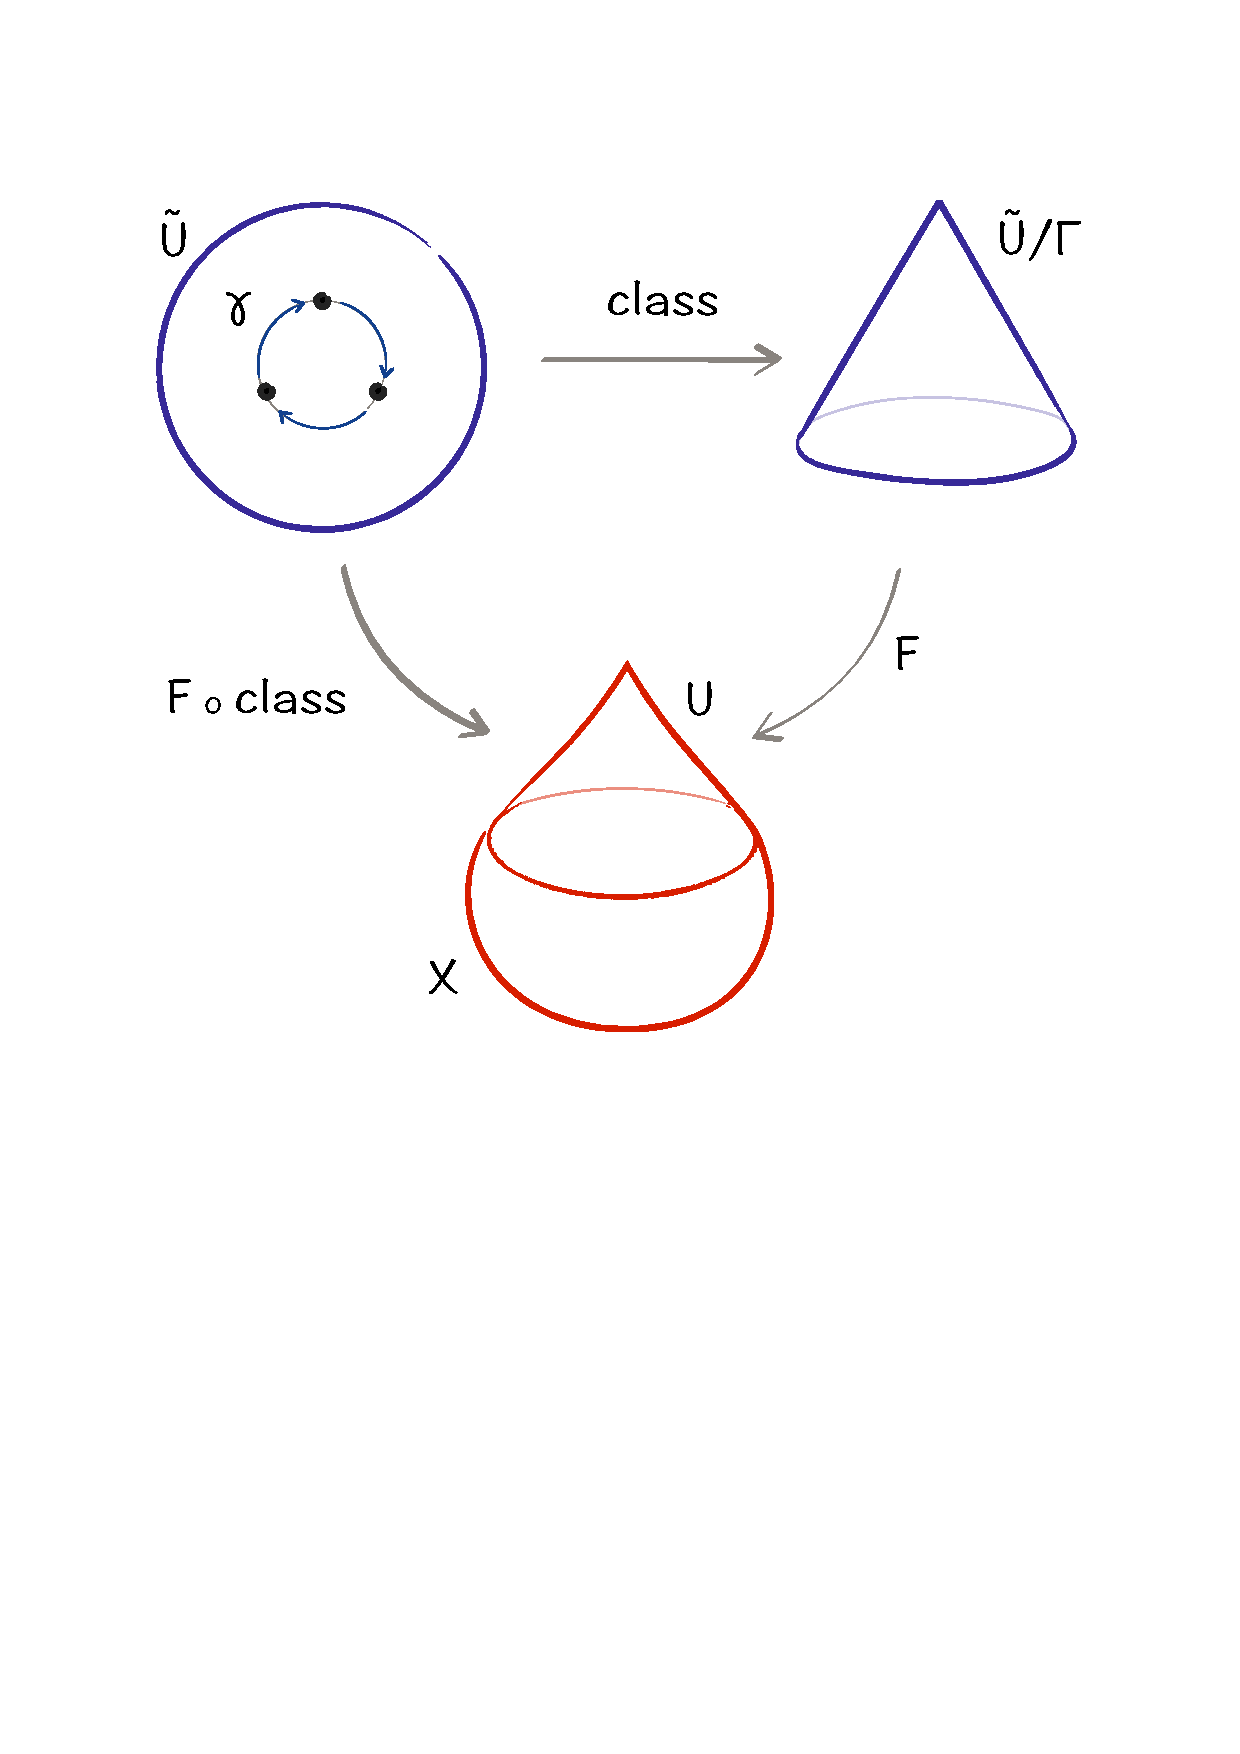
\includegraphics[width=.50\textwidth]{Figures/fig-D-orbifold.pdf}}
  \caption{Generating Family for a D-orbifold.}
  \label{D-orbifold}
\end{figure}
%%###########

\begin{Article}{Linear action or not?}{}
  In the previous definition,
  it is equivalent to ask $\Gamma$ to be a finite group of diffeomorphisms or to be linear.
  Indeed,
  we define a $\Gamma$-invariant Riemannian metric by
  $$
    \langle u,v \rangle_\Gamma = {1 \over \# \Gamma} \sum_{\gamma \in \Gamma} \langle \gamma u,\gamma v \rangle,
  $$
  then the {\em slice theorem} states that this action is equivalent to an orthogonal action.
\end{Article}

\begin{Article}{Example: The simplest.}{}
  It is important to clarify a similar point we made for the diffeological definition of manifold.
  Here again a D-orbifold comes \emph{a priori} as a diffeological space,
  that is,
  equipped with a diffeology $\cD$.
  The fact that $X$ is an orbifold is a property of the diffeology,
  not the set itself,
  as the following examples will show.

  The first example,
  the simplest,
  is certainly $\Delta_1 = \RR /\{\pm 1\}$,
  which is equivalent to the half-line $\LeftClosedInterval{0,\infty}$ equipped with the pushforward of the standard diffeology of $\RR$ by the map $x \mapsto x^2$.
  The D-topology is the subset topology on $\LeftClosedInterval{0,\infty}$.
  A plot of $\Delta_1$ is a positive parametrization that can be written locally everywhere as some $r \mapsto Q(r)^2$.
\end{Article}

\begin{Article}{Example: The cone orbifold.}{}
  Not the simplest example but the most known is the cone orbifold.
  It is defined as the quotient of the complex number space $\CC$ by a cyclic group $\cU_m$.
  We denote it by:
  $$
    \cC_m = \CC/\cU_m,
  $$
  where $m \in \NN$,  $m\neq 0$ and
  $$
    \cU_m = \{ \exp(2i\pi k/m) \mid k = 1 \dots m \}.
  $$
  The diffeological space $\cC_m$,
  equipped with the quotient diffeology,
  is by definition an orbifold.
  The topologists are used to represent this orbifold by gluing the two sides of a fundamental domain,
  as it is illustrated in Figure \ref{fig-cone}.
  But that representation obscures the diffeological intuition.
  \uline{We will show now how the orbifold $\cC_m$ can be represented as a special diffeology on the field $\CC$ itself.}

  \begin{figure}[ht]
    \centerline{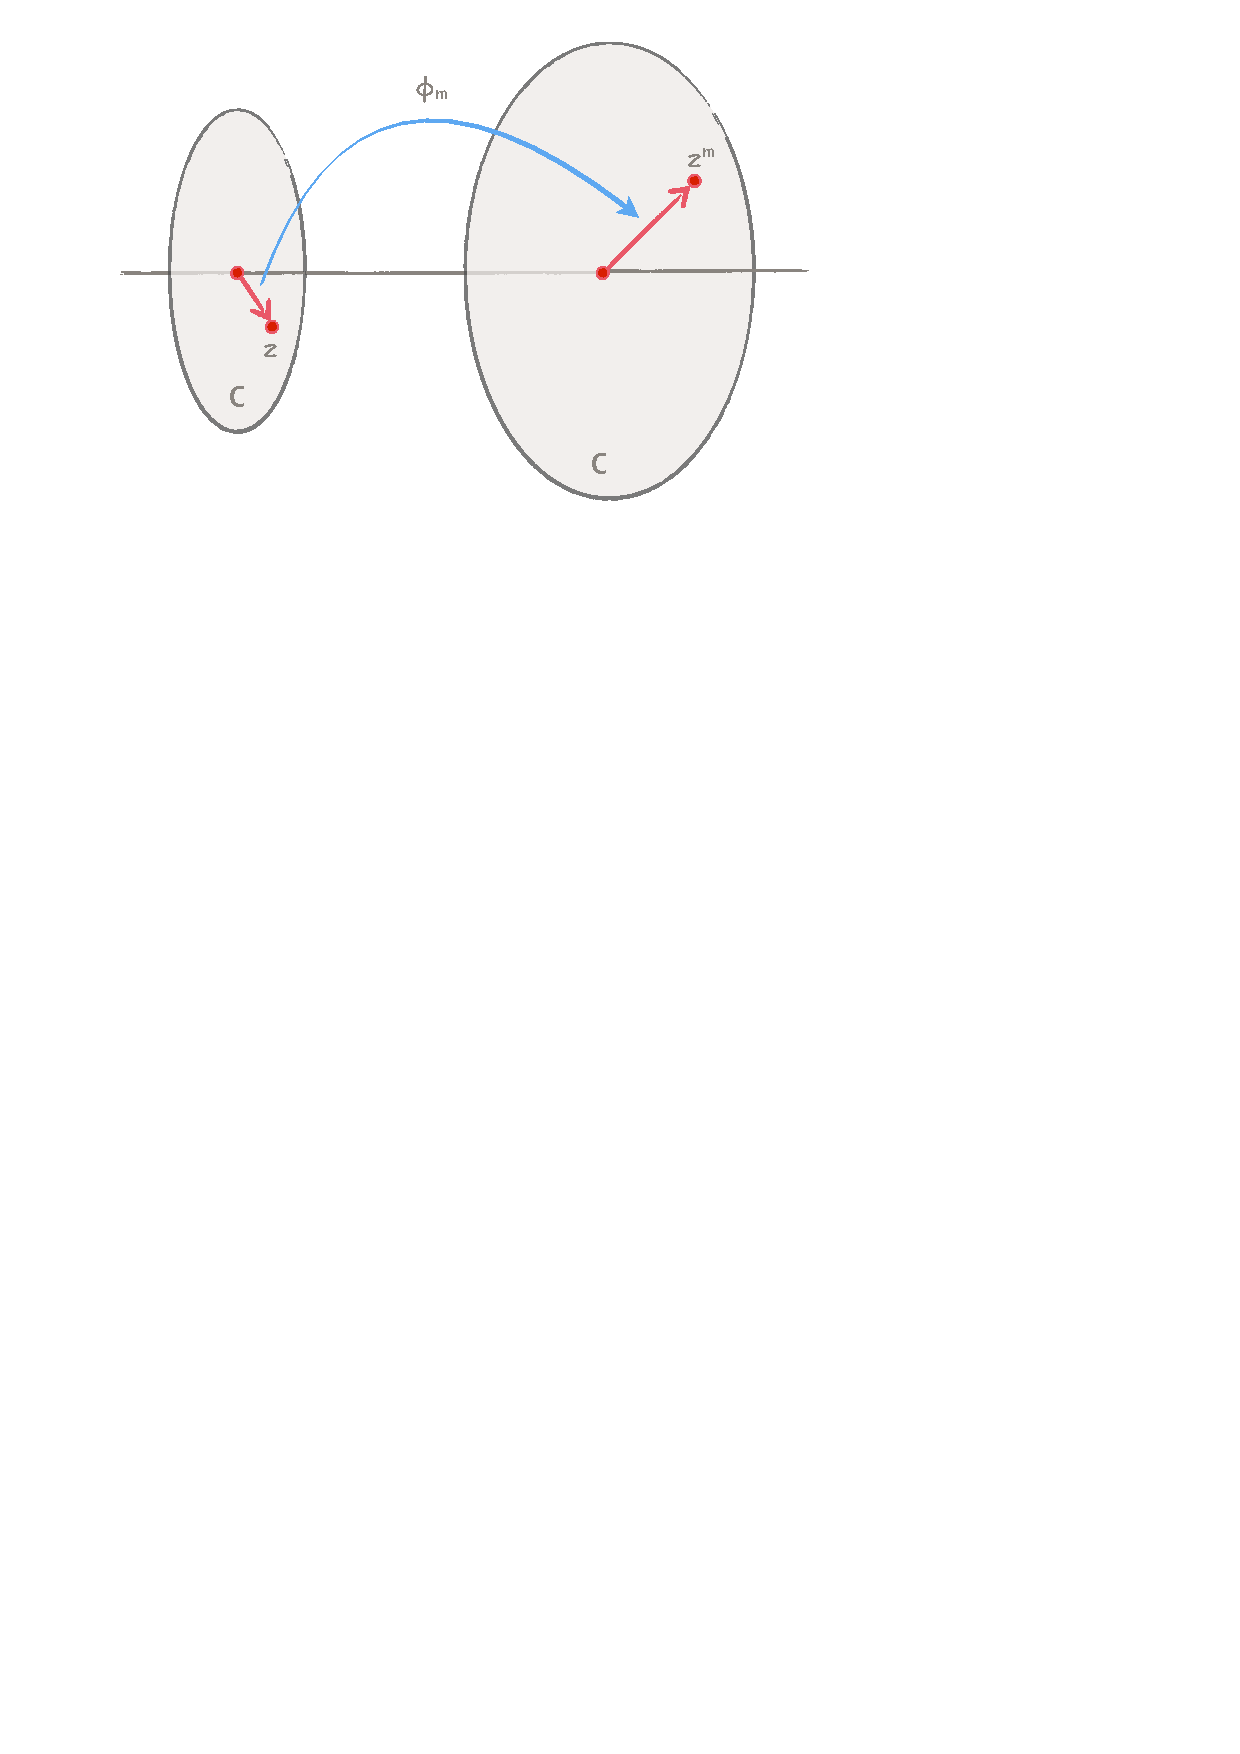
\includegraphics[width=0.70\textwidth]{Figures/DiffCone.pdf}}
    \caption{\small The cone orbifold viewed by a diffeologist.}
    \label{fig-diffcone}
  \end{figure}

  Considering then the map
  $$
    \pphi_m : \CC \to \CC \quad \mbox{with} \quad \pphi_m(z) = z^m,
  $$
  it is clear that the preimages of the points $\zeta \in \CC$ are exactly the orbits of the group $\cU_m$.
  Since $\pphi_m$ is surjective,
  $\CC$ can be identified with the quotient set $\CC/\cU_m$,
  with canonical projection $\pphi_m$.
  The last question is what diffeology on $\CC$ represents the quotient diffeology?
  Naturally, the answer is the pushforward
  $$
    \cC^\infty_m=\pphi_{m*}(\cC^\infty)
  $$
  of the standard diffeology $\cC^\infty$ on $\CC$.
  Note that the D-topology of $\cC^\infty_m$ is still the standard topology of $\CC$.

  A parametrization $P : U \to \CC$ belongs to $\cC^\infty_m$ if and only if,
  for all point $r_0 \in U$,
  there exists a small ball $B$ centered at $r_0$ and a smooth parametrization $Q : B \to \CC$ such that $P(r) = Q(r)^m$,
  for all $r \in B$.

  Actually,
  if $P(r_0) \neq 0$,
  it is sufficient to ask $P$ to be smooth on some small ball around $r_0$,
  and if $P(r_0)=0$,
  then there is no shortcut,
  we have to find $Q$ satisfying the condition above.

  Thus,
  as we can see in this simple example,
  the same set $\CC$ can be equipped with an infinity of orbifold diffeologies,
  one for each integer,
  without altering the underlying space.
\end{Article}

\begin{Article}{Example: The waterdrop.}{}
  This orbifold,
  the waterdrop drawn in the many figures above,
  is a diffeology defined on the sphere $\Sph^2$.
  %%###########
  % MARK: Figure
  %%###########
  \begin{figure}[htb]
    \centerline{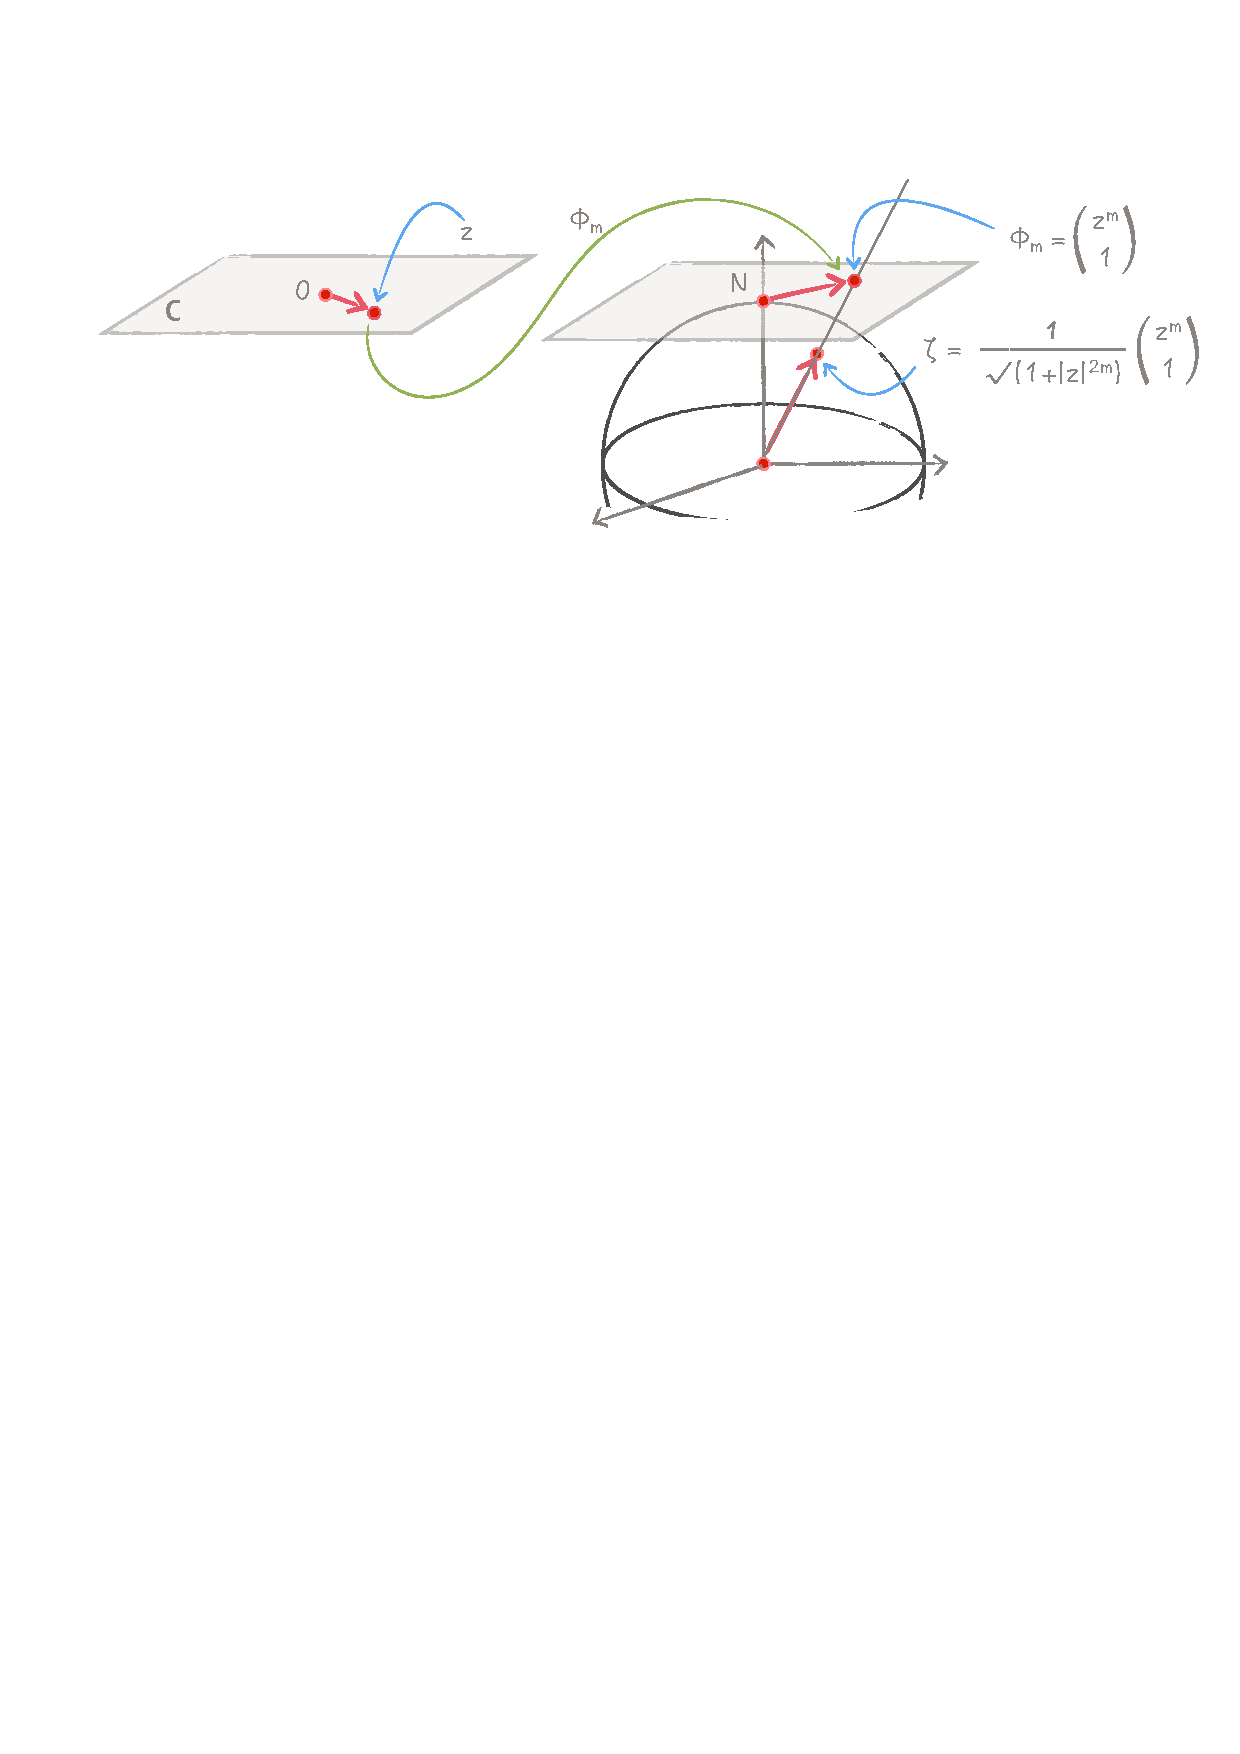
\includegraphics[width=1\textwidth]{Figures/fig-Teardrop.pdf}}
    \caption{The waterdrop Orbifold.}
\label{Teardrop}
  \end{figure}
  %%###########
  For convenience,
  $\Sph^2$ is regarded as a subset of $\CC \times \RR$.
  A plot of the \emph{waterdrop diffeology} is a smooth parametrization $\zeta$ in $\Sph^2$ which is identified to $\CC \times \RR$,
  with $N = (0,1)$ the \emph{North Pole},
  satisfying:
  $$
    \zeta : U \to \CC \times \RR
    \SpacedText{with}
    \left\{
    \begin{array}{l}
    \zeta(r) = \begin{pmatrix}z(r) \\ t(r) \end{pmatrix}, \\[1em]
    |z(r)|^2 + t(r)^2 =1.
    \end{array}
    \right.
  $$
  such that,
  for all $r_0 \in U$:

  \noindent$\bullet$ if $\zeta(r_0) \neq N$,
  then there exists a small ball $B$ centered at $r_0$ such that $\zeta \restriction B$ is smooth.

  \noindent$\bullet$ If $\zeta(r_0)=N$,
  then there exists a small ball $B$ centered at $r_0$ and a smooth parametrization $z$ in $\CC$ defined on $B$ such that,
  for all $r\in B$,
  $$
    \zeta(r) = {1 \over \sqrt{1 + |z(r)|^{2m}}}\begin{pmatrix} z(r)^m \\ 1 \end{pmatrix}.
  $$
  \noindent\uline{Note that} this orbifold diffeology on $\Sph^2$ is a \emph{subdiffeology} of the standard diffeology of manifold,
  embedded in $\RR^3$.

  \noindent\uline{Note also} how it is possible to multiply the number of conical points on the sphere.
\end{Article}

\begin{Article}{Example: The hedgehog.}{}
  After the cone which has a unique singularity,
  of conic type and structure group $\cU_m$,
  at the north pole,
  it is not hard to imagine many other examples based on the construction of previous two:
  a sphere,
  or a plane,
  with as many different singular conic (or not) points we want.
  The fact that,
  contrarily to manifolds,
  orbifolds may have a rich set of smooth local invariants,
  allows us to build easily more different orbifold structures on the same underlying space.
  In our examples above,
  we just picked up a diffeology finer than the standard manifold diffeology which happens to be an orbifold diffeology.

  \begin{figure}[bht]
    \centerline{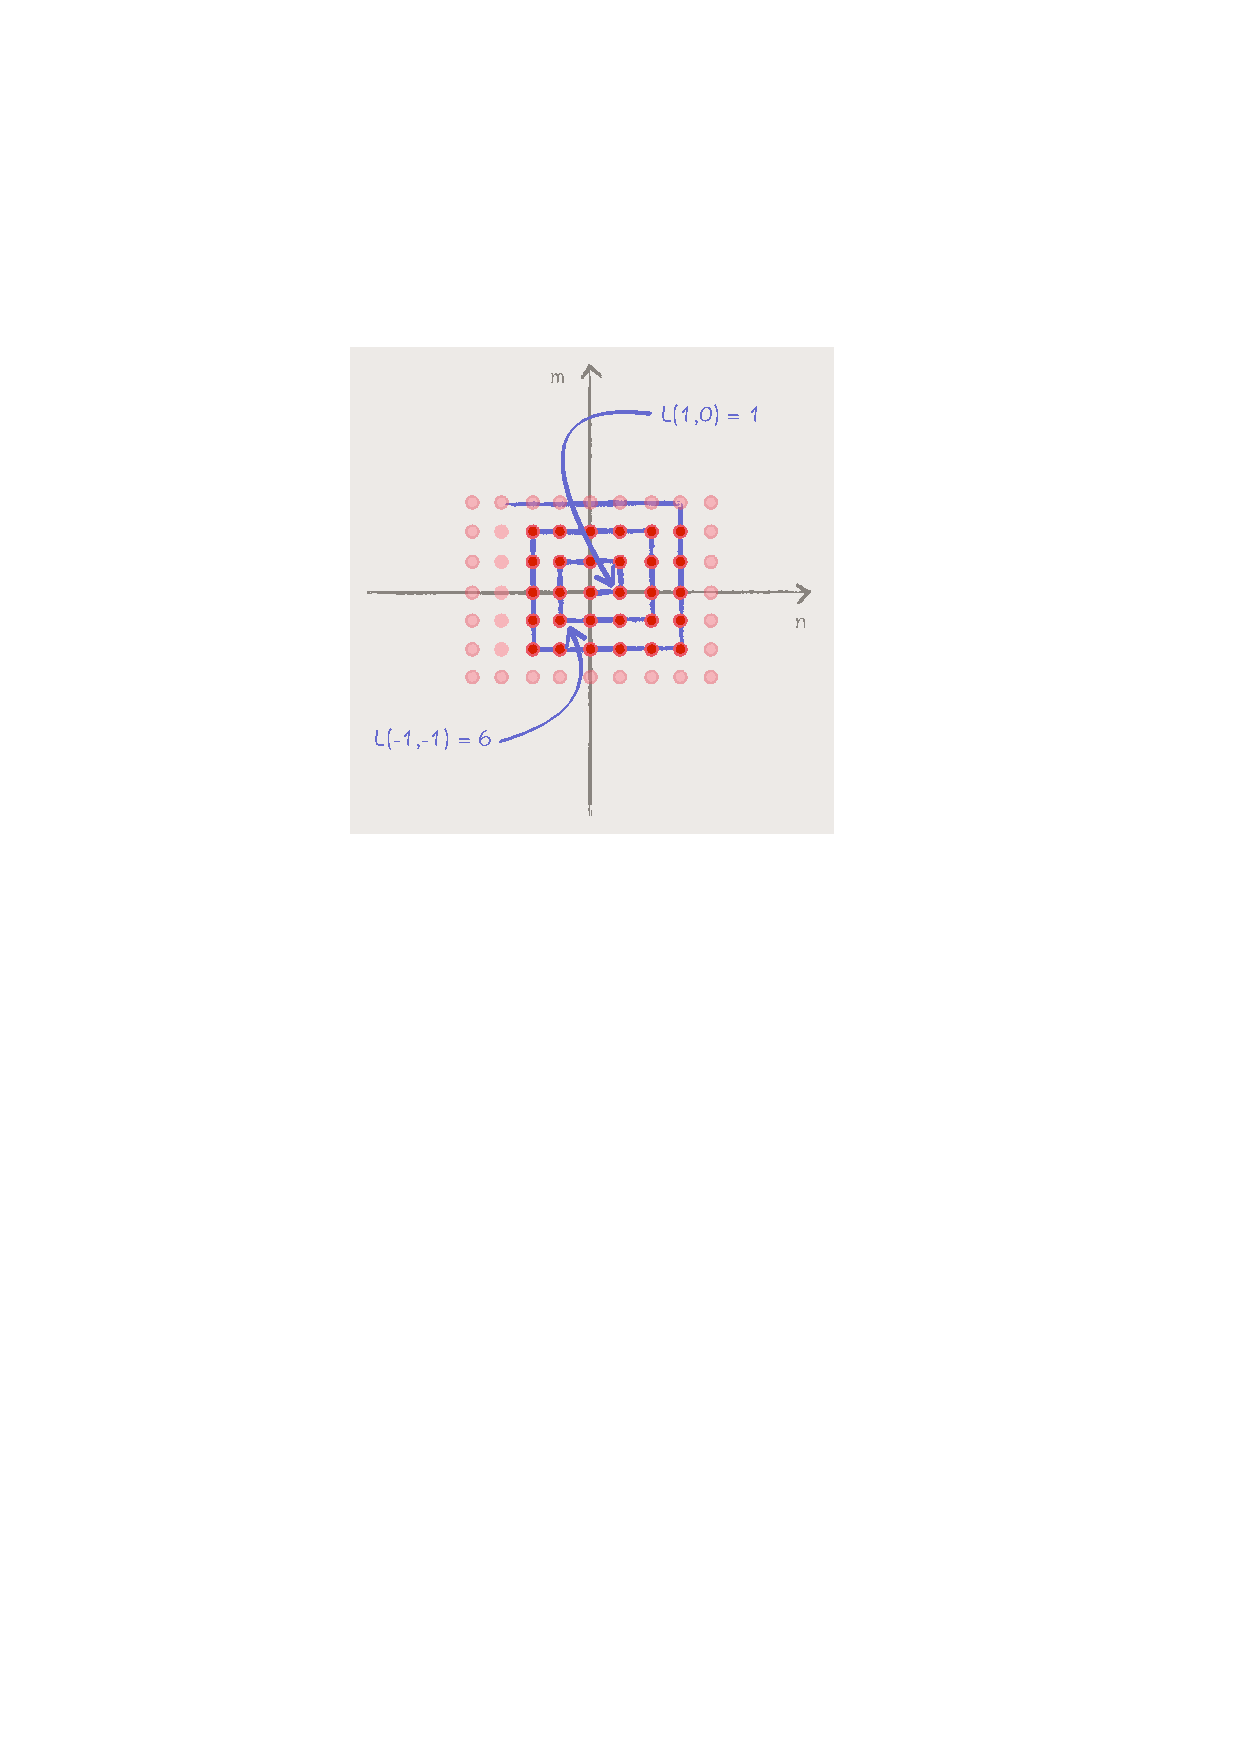
\includegraphics[width=.5\textwidth]{Figures/L(n,m).pdf}}
    \caption{\small The function $L(n,m)$.}
    \label{fig-L(n,m)}
  \end{figure}

  In particular,
  we have seen earlier that the quotient space of a disc by $\cU_m$ is equivalent to the same disc but equipped with a finer diffeology.
  It is then easy to extract from a manifold diffeology,
  a finer orbifold diffeology with as many conic singularities as we want,
  with arbitrary structure groups.
  Let's build a simple example:
  Consider the plane $\CC$ and let $L : \ZZ +i\ZZ \to \NN$ be the bijection described in Figure \ref{fig-L(n,m)}.

  Then,
  let us define the following diffeology,
  with parametrizations $\zeta:U\to \CC$ such that,
  for all $r_0 \in U$:

  \begin{enumerate}
    \item if $\zeta(r_0) \not\in \ZZ +i\ZZ$,
    then there exists a small ball $B$ centered at $r_0$ such that $\zeta \restriction B$ is smooth.
    \item If $\zeta(r_0) = n+im$,
    with $n,m\in \ZZ$,
    then there exists a small ball $B$ centered at $r_0$ and a smooth parametrization $z$ in $\CC$ defined on $B$ such that,
    for all $r\in B$,
    $$
      \zeta(r) = n+im + z(r)^{1+L(n,m)}.
    $$
  \end{enumerate}

  In this example, the integer points $n+im \in \CC$ are conic with cyclic groups,
  all different,
  equal to $\ZZ_{1+L(n,m)}$.

  It should be noted that,
  with all the transition functions,
  a description of this orbifold using the original Satake's defining families,
  would be,
  for the least,
  laborious.
  We can appreciate,
  on this example,
  the simplification brought by the diffeological approach.
\end{Article}

\begin{Article}{Smooth Maps Between Orbifolds.}{}
  \label{Smooth-Maps-Between-Orbifolds}
  Let us continue with the cone orbifold $\cC_m = \CC/\cU_m$.
  Let $f \colon \RR^2 \to \RR^2$ be defined by
  $$
    f(x,y) = \begin{cases}
    0 & \text{ if } r > 1 \text{ or } r = 0 \\[1ex]
    e^{-1/r} \rho_n(r) (r,0) & \text{ if } \frac{1}{n+1} < r \leq \frac{1}{n}
    \text{ and $n$ is even } \\[1ex]
    e^{-1/r} \rho_n(r) (x,y) & \text{ if } \frac{1}{n+1} < r \leq \frac{1}{n}
    \text{ and $n$ is odd},
    \end{cases}
  $$
  where $r = \sqrt{x^2 + y^2}$ and $\rho_n$ is a function vanishing flatly outside the interval $\OpenInterval{1/(n+1),1/n}$ and not inside,
  see Figure \ref{function-rho}.
  \begin{figure}[htb]
    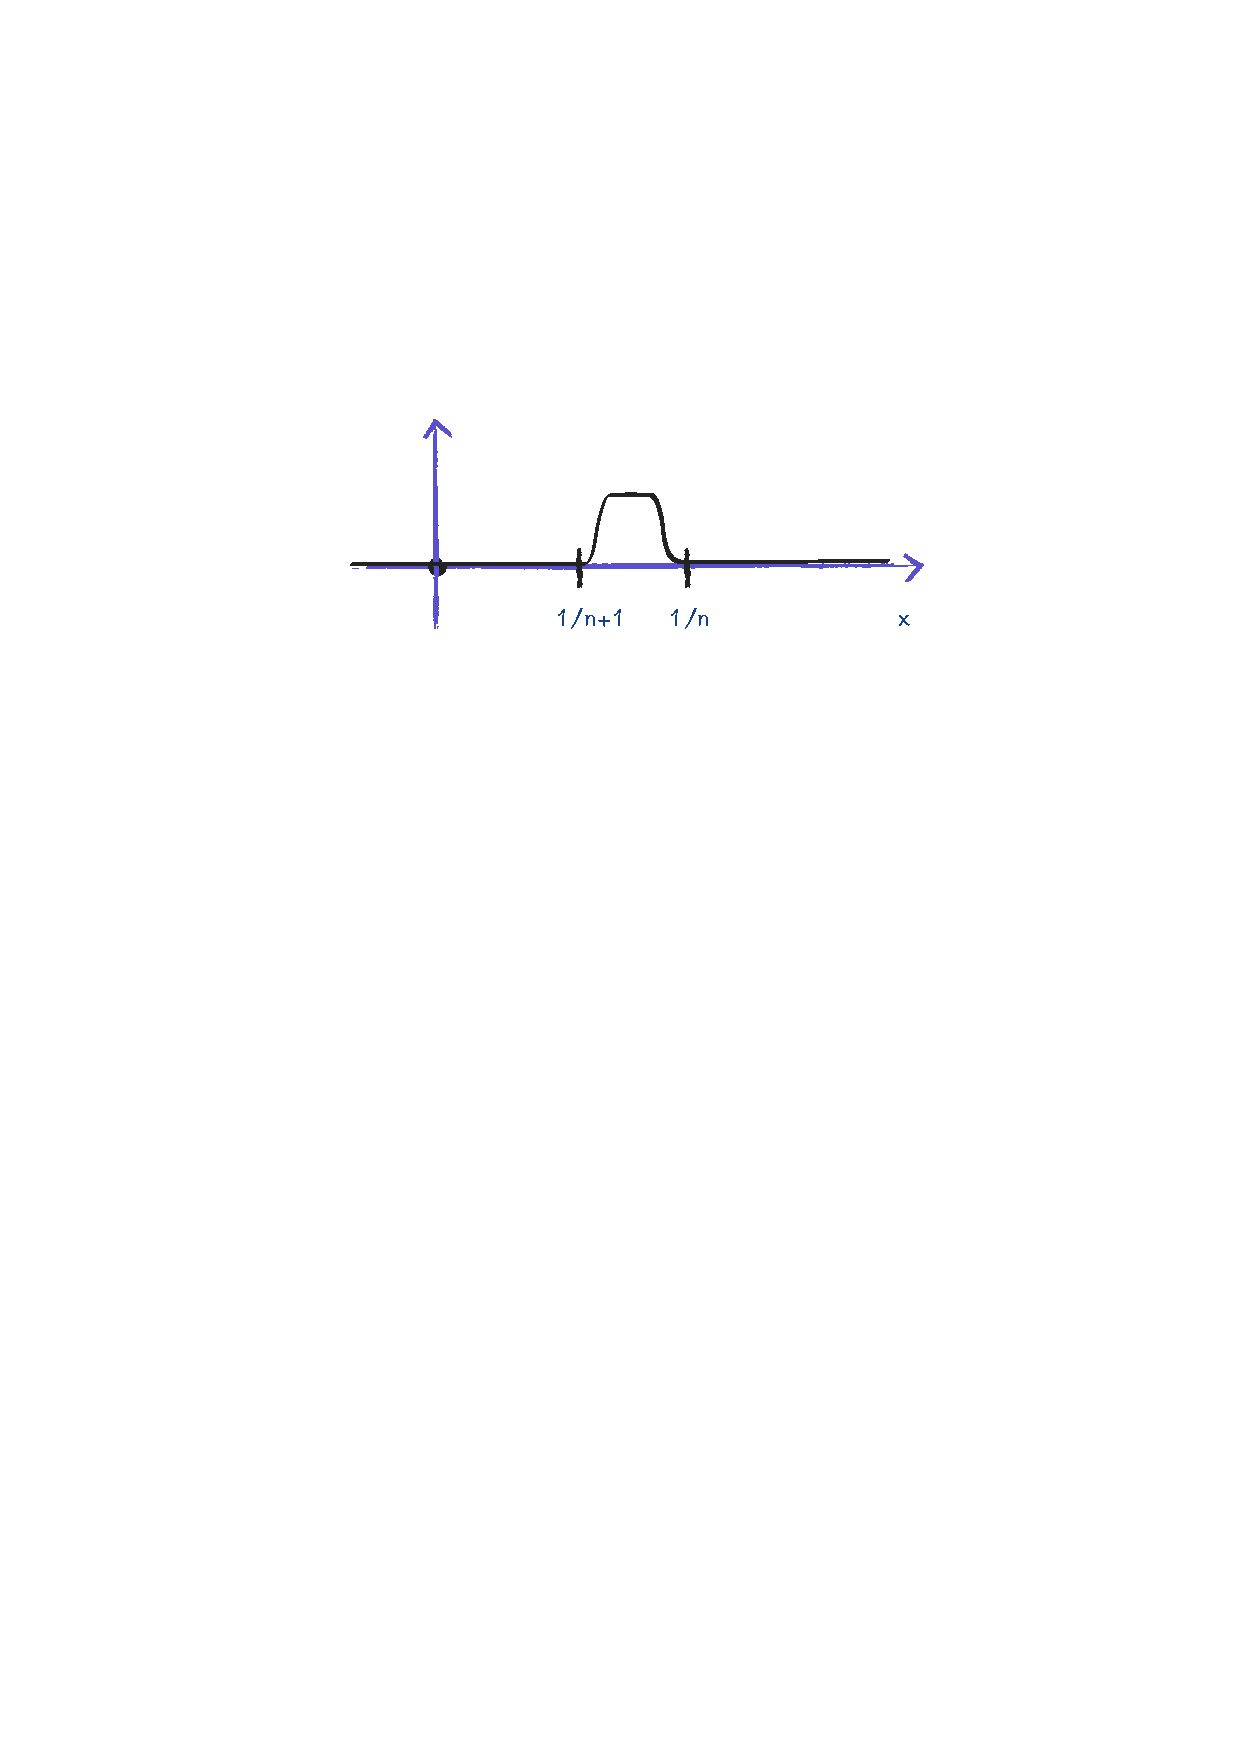
\includegraphics[width=.50\textwidth]{Figures/fig-function-rho.pdf}
    \caption{The function $\rho_n$.}
    \label{function-rho}
  \end{figure}
  Remark now that
  $$
    f(AX) = h_X(A) f(X),
    \SpacedText{with}
    X \in \RR^2
    \SpacedText{and}
    A \in \SO(2).
  $$
  On the annulus
  $$
    \frac{1}{n+1} < r \leq \frac{1}{n},
    \SpacedText{with}
    \left\{
    \begin{array}{ll}
    h_X(A) = \Id_{\RR^2} & \text{if $n$ is even, and} \\[1ex]
    h_X(A) = A & \text{if $n$ is odd.}
    \end{array}
    \right.
  $$
  Now,
  the function $f$ descends onto a smooth map $\varphi$ from the cone orbifold $\cC_m$ to itself.
  In particular because the homomorphism $h_X$ flips from the identity to trivial on any successive annulus,
  $\varphi$ has no local equivariant smooth lifting.

  This is a big difference with diffeomorphisms for which it is proven that the stabilizer of one point is locally mapped equivariantly into the stabilizer of the image by a homomorphism.
  \begin{center}
    \begin{tikzpicture}[every node/.style={midway}]
      \matrix[column sep={10em,between origins}, row sep={2.5em}] at (0,0) {
      \node(A) {$\RR^2$}  ; & \node (B) {$\RR^2$}; \\
      \node(C) {$\cC_m = \RR^2/\cU_m$};             & \node (D) {$\cC_m = \RR^2/\cU_m$};\\
      };
      \draw[->] (A) -- (B) node[auto=left]  {$f$};
      \draw[->] (A) -- (C) node[auto=right]  {$\Class_m$};
      \draw[->] (B) -- (D) node[auto=left] {$\Class_m$};
      \draw[->] (C) -- (D) node[auto=right] {$\varphi$};
    \end{tikzpicture}
  \end{center}
  This example is the very illustration of the unsuccessful attempt to define smooth maps between orbifolds as locally equivariant maps,
  on the level of local symmetry group,
  and that answers Satake's footnote in \cite[page 469]{Sat57},
  \begin{quote}
    ``{\itshape The notion of $\Cinfty$-map thus defined is inconvenient in the point that a composite of two $\Cinfty$-maps defined in a different choice of defining families is not always a $\Cinfty$ map.}''
  \end{quote}
  Embedding of orbifolds into a category such as \{Diffeology\} could have solved this question.
  The existence of good smooth maps between orbifolds is crucial for having a covariant satisfactory theory of orbifolds.
\end{Article}

%%%%%%%%%%%%%%%%%%%%%%%%%%%%%%%%%%%%%%%%%%%%%%%%%%%%%%%%%%
%%
%% MARK:  Equivalence between V-Manifolds and D-orbifolds
%%
%%%%%%%%%%%%%%%%%%%%%%%%%%%%%%%%%%%%%%%%%%%%%%%%%%%%%%%%%%
\section{Equivalence between V-manifolds and D-orbifolds}

\begin{Article}{V-manifolds are D-orbifolds.}{}
  \label{V-manifolds-are-D-orbifolds}
  Let $M$ be a Hausdorff topological space.
  A defining family $\cF$ on $M$ determines a diffeology of orbifold.
  Namely,
  the diffeology generated by the parametrizations $\varphi\colon\tilde U\to U$,
  for all $(\tilde U,G,\varphi) \in \cF$.
\end{Article}

\begin{Article}{Equivalence of defining families.}{}
  Let $M$ be a Hausdorff topological space.
  If two defining families $\cF$ and $\cF'$ on $M$ generate the same diffeology
  then they are equivalent.
  More precisely,
  the union $\cF'' = \cF \cup \cF'$ is a defining family.
\end{Article}

\begin{Article}{D-orbifolds are V-manifolds.}{}
  Conversely,
  let $X$ be a D-orbifold,
  then equip $X$ with the D-topology (assumed Hausdorff).
  Let $\cA$ be an atlas of $X$,
  the strict generating family of the atlas $\cA$ is a defining family in the sense of Satake,
  and equip $X$ with a structure of V-manifold for its D-topology.

  Two different atlases $\cA$ and $\cA'$ give equivalent Satake defining families,
  essentially because they are sub-atlases of the maximal atlas.
\end{Article}

\begin{Article}{Equivalence of definitions.}{}
  The two constructions above are,
  up to an equivalence,
  inverse one from each other.

  \uline{Note.} Actually,
  Satake defined only what we call \emph{reflexion free V-manifolds}.
  But there was no technical obstacles to extend the definition to any V-manifold.
\end{Article}


%%%%%%%%%%%%%%%%%%%%%%%%%%%%%%%%%%%%%%%%%%%%%%%%%%%%%%%%%%
%%
%% MARK:  Internal Structure of a D-orbifold
%%
%%%%%%%%%%%%%%%%%%%%%%%%%%%%%%%%%%%%%%%%%%%%%%%%%%%%%%%%%%
\section{Internal structure of a D-orbifold}

% The proofs of these late propositions are consequence of the precise description of what we can call now the \emph{internal structure} of a D-orbifold.

\begin{Article}{The groupoid $\GG$ of germs of local diffeomorphisms.}{}
  Let $X$ be any diffeological space.
  We define the groupoid $\GG$ of \emph{germs of local diffeomorphisms} of $X$ as follows:
  $$
    \left\{
    \begin{array}{rcl}
    \Obj(\GG) & = & X, \\[.5ex]
    \Mor(\GG) & = & \{\ \germ(\varphi)_x \mid \varphi \in \Diff_\loc(X) \mbox{ and } x \in \Domain(\varphi) \}.
    \end{array}
    \right.
  $$
  The \emph{source} maps,
  the \emph{target} maps and the composition of germs of local diffeomorphisms are defined as follows:

  $$
    \left\{
    \begin{array}{l}
    \Src(\germ(\varphi)_x) = x, \quad \Trg(\germ(\varphi)_x) = \varphi(x). \\[.5ex]
    \germ(\varphi)_x \cdot \germ(\varphi')_{x'} = \germ(\varphi' \circ \varphi)_x, \text{ with } x'=\varphi(x).
    \end{array}
    \right.
  $$

  The pseudogroup of local diffeomorphisms of $X$ is equipped with the functional diffeology of pseudogroup,
  that is,
  the diffeology of local smooth map for the pairs $(f,f^{-1})$,
  where $f \in \Diff_\loc(X)$.
  Let then define the $\germ$ map by:
  $$
    \left\{
    \begin{array}{l}
    \fG = \{ (\varphi,x) \mid \varphi \in \Diff_\loc(X) \mbox{ and } x \in \Domain(\varphi) \}. \\[.5ex]
    \germ : (\varphi,x) \mapsto \germ(\varphi)_x.
    \end{array}
    \right.
  $$
  We equip $\Mor(\GG)$ with the {\itshape pushforward} of the diffeology of $\fG$ by the map $\germ$.
  That makes $\GG$ a diffeological groupoid.
  That means essentially that:

  (a) the multiplication and the inversion are smooth maps

  (b) and the inclusion $\Obj(\GG) \hookrightarrow \Mor(\GG)$ by the identities is an induction.
\end{Article}

\begin{Article}{The structure groupoid of an orbifold.}{}
  Let $X$ be an $n$-orbifold,
  $\cA$ be an atlas,
  $\cF$ be the strict generating family over $\cA$,
  $\cN$ be the nebula and $\Eval$ be the evaluation map,
  that is:
  $$
    \cN = \displaystyle{\coprod_{F \in \cF} \Domain(F)}
    \SpacedText{and}
    \Eval : \cN \to X \SpacedText{with} \Eval(F,r) = F(r).
  $$

  %%###########
  % MARK: Figure
  %%###########
  \begin{figure}[htb]
    \centerline{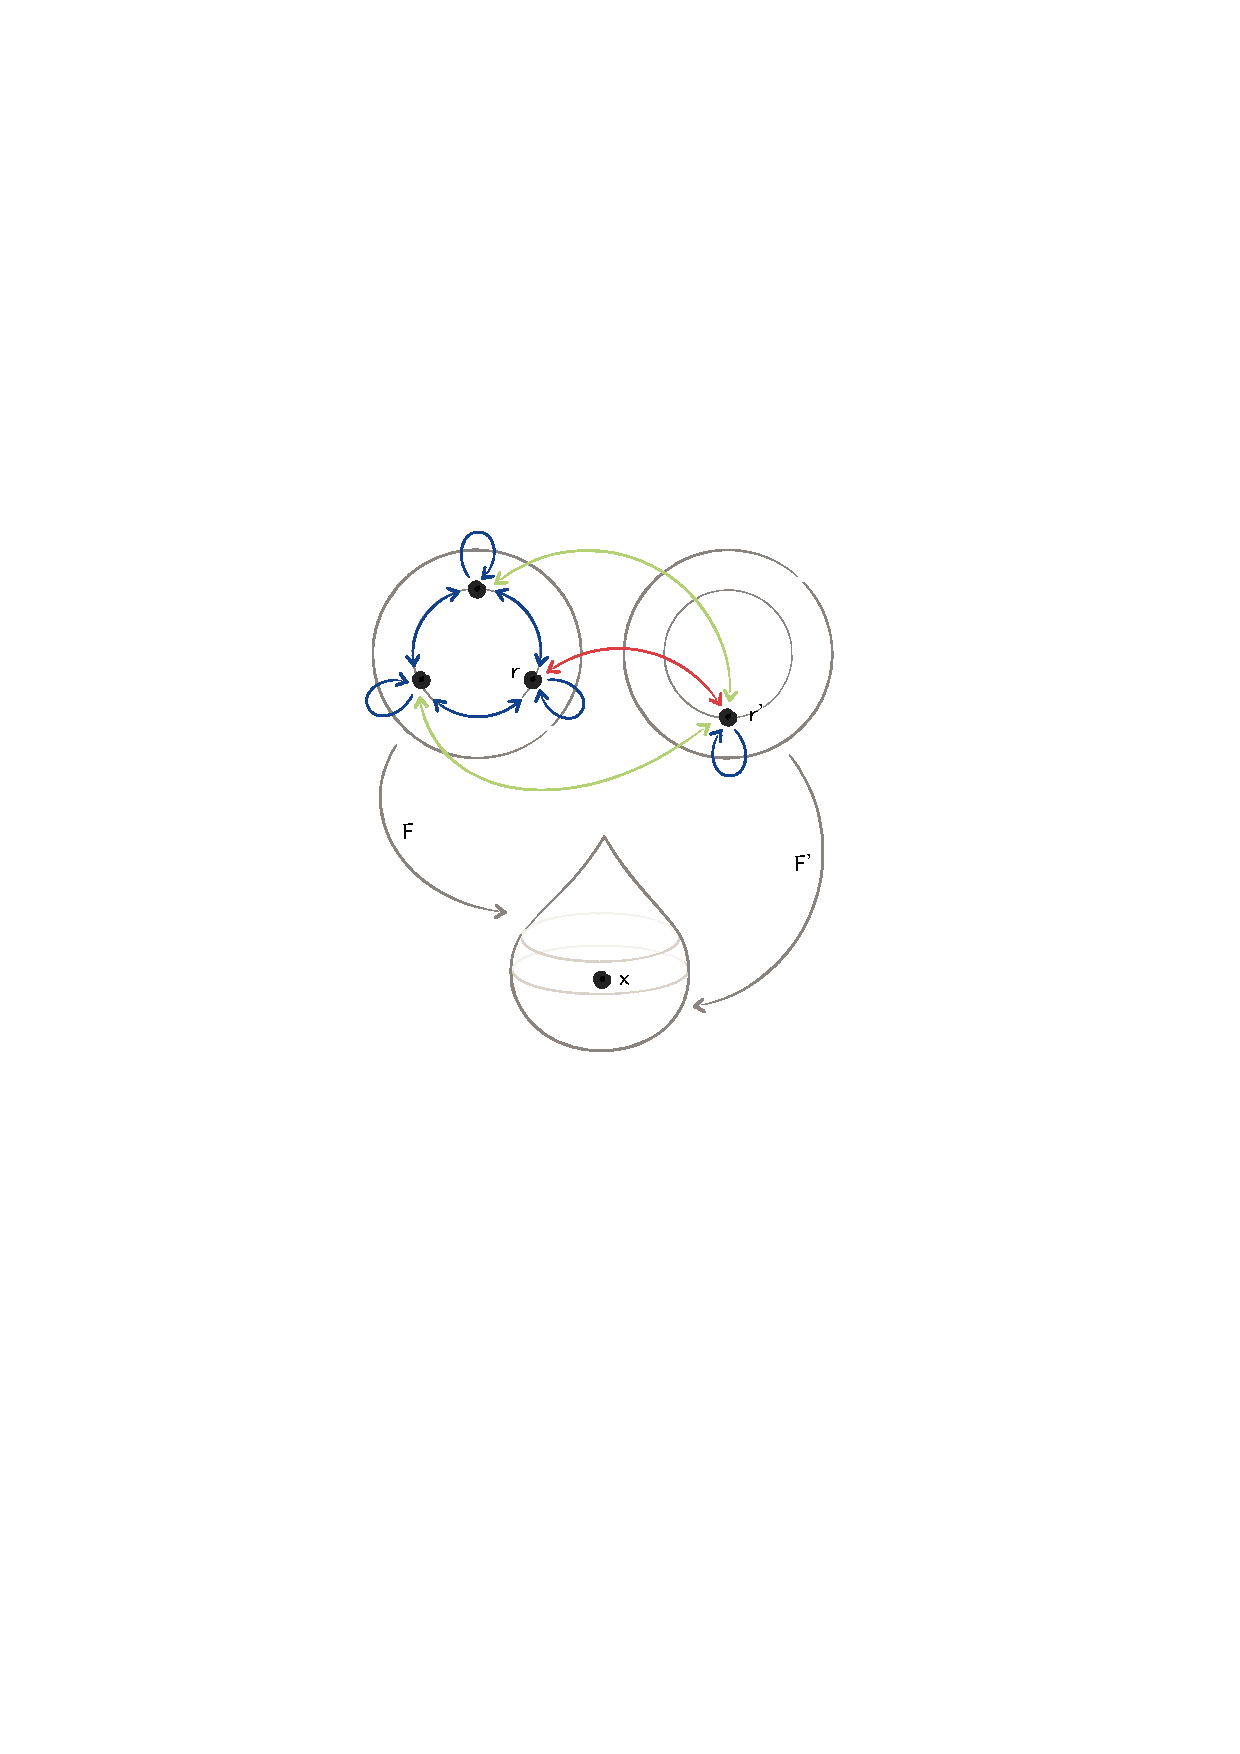
\includegraphics[width=.5\textwidth]{Figures/fig-Assembling-groupoid.pdf}}
    \caption{The Groupoid of the Teardrop.}
    \label{Assembling-groupoid}
  \end{figure}
  %%###########

  We call \emph{Structure groupoid} $\GG$ of the orbifold $X$ the subgroupoid of the groupoid of germs of local diffeomorphisms of $\cN$ that descends on the identity of $X$ along $\Eval$.
  That is,
  $$
    \Mor_{\GG}((F,r),(F',r')) =
    \left\{ \left.
    \vphantom{\begin{array}{l}
    \varphi \in \Diff_\loc(\RR^n) \\
    F' \circ \varphi = F \restriction \Domain(\varphi)
    \end{array}}
    \germ(\varphi)_r \right | \right.
    \left.
    \hspace{-1ex}\begin{array}{l}
    \varphi \in \Diff_\loc(\RR^n), r'=\varphi(r)  \\
    F' \circ \varphi = F \restriction \Domain(\varphi)
    \end{array}
    \right\}
  $$

  \uline{Note.} In order to show the dependency of the structure groupoid with respect to the atlas $\cA$ we need the two following lemmas.
\end{Article}

\begin{Article}{Lifting the identity.}{}
  \label{Lifting-The-Identity}
  Let $\cQ = \RR^n\!/\Gamma$.
  Consider a local smooth map $F$ from $\RR^n$ to itself,
  such that $\Class \circ F = \Class$.
  In other words,
  $F$ is a local lifting of the identity on $\cQ$.
  Then,
  %
  \begin{center}
    \begin{tikzcd}[column sep=1cm, row sep=1cm,every label/.append style = {font = \small}]
      \RR^n \supset \tilde U \arrow[dr, swap, "\Class"]  \arrow[rr, "F"] &     &  \RR^{n} \arrow[dl,"\Class"] \\
      & \cQ &
    \end{tikzcd}
  \end{center}
  %
  \uline{Theorem.} {\itshape $F$ is locally equal to some group action $F(r) =_\loc \gamma \cdot r$,
  where $\gamma \in \Gamma$.}
  %
\end{Article} % Lifting The Identity

\begin{proof}
  Let us assume first that $F$ is defined on an open ball $B$.
  Then,
  for all $r$ in the ball,
  there exists a $\gamma \in \Gamma$ such that $F(r) = \gamma\cdot r$.
  Next,
  for every $\gamma \in \Gamma$, let
  $$
    F_\gamma \colon B \to \RR^n \times \RR^n \quad \mbox{with} \quad F_\gamma(r) = (F(r), \gamma\cdot r).
  $$
  Let $\Delta \subset \RR^n \times \RR^n$ be the diagonal and let us consider
  $$
    \Delta_\gamma = F_\gamma^{-1}(\Delta) = \{ r \in B \mid F(r) = \gamma\cdot r \}.
  $$
  \uline{Lemma 1.} {\itshape There exist at least one $\gamma \in \Gamma$ such that the interior $\mathring{\Delta}_\gamma$ is non-empty.}

  $\blacktriangleleft$~Indeed,
  since $F_\gamma$ is smooth (thus continuous),
  the preimage $\Delta_\gamma$ by $F_\gamma$ of the diagonal is closed in $B$.
  However,
  the union of all the preimages $F_\gamma^{-1}(\Delta)$
  ---~when $\gamma$ runs over $\Gamma$~---
  is the ball $B$.
  Then,
  $B$ is a finite union of closed subsets.
  According to Baire's theorem,
  there is at least one $\gamma$ such that the interior $\mathring{\Delta}_\gamma$ is not empty.~$\blacktriangleright$

  \uline{Lemma 2.}~{\itshape The union $\mathring{\Delta}_\Gamma = \cup_{\gamma \in \Gamma} \mathring{\Delta}_\gamma$ is an open dense subset of $B$.}

  $\blacktriangleleft$~Indeed,
  let $B' \subset B$ be an open ball.
  Let us denote with a prime the sets defined above but for $B'$.
  Then,
  $\Delta'_\gamma = (F_\gamma  \restriction B' )^{-1}(\Delta) = \Delta_\gamma \cap B'$,
  and then $\mathring{\Delta}'_\gamma = \mathring{\Delta}_\gamma \cap B'$.
  Thus,
  $B' \cap \mathring{\Delta}_\Gamma  = B' \cap (\cup_{\gamma \in \Gamma} \mathring{\Delta}_\gamma) = \cup_{\gamma \in \Gamma} \mathring{\Delta}'_\gamma$,
  which is not empty for the same reason that $\cup_{\gamma \in \Gamma} \mathring{\Delta}_\gamma$ is not empty.
  Therefore,
  $\mathring{\Delta}_\Gamma$ is dense.~$\blacktriangleright$

  In conclusion:
  the tangent linear map $\Der(F) \colon B \to \GL(n,\RR)$ is smooth,
  then continuous,
  thus $\Der(F)^{-1}(\Gamma)$ is closed.
  But,
  $\mathring{\Delta}_\Gamma$,
  which is an open dense subset of $B$,
  is contained in $\Der(F)^{-1}(\Gamma)$.
  Hence,
  $B$ is contained in $\Der(F)^{-1}(\Gamma)$ (its own closure) which is contained in $B$.
  Thus,
  $\Der(F)^{-1}(\Gamma) = B$.
  Then,
  since $B$ is connected, $\Der(F)(B) \subset \Gamma$ is connected.
  But $\Gamma \subset \GL(n,\RR)$ is discrete,
  then $\Der(F)(B) = \{ \gamma \}$,
  for some $\gamma \in \Gamma$.
\end{proof}


\begin{Article}{Lifting local diffeomorphisms.}{}
  \label{Lifting-Local-Diffeomorphisms}
  Let $\cQ = \RR^n\!/\Gamma$ and $\cQ' = \RR^{n'}\!/\Gamma'$,
  Then,

  \uline{Theorem.} {\itshape Every local smooth lifting $\tilde f$ of any local diffeomorphism $f$,
  from $\cQ$ to $\cQ'$,
  is necessarily a local diffeomorphism,
  from $\RR^n$ to $\RR^{n'}$.
  In particular $n = n'$.
  %
  Moreover,
  let
  $$
    x \in \Domain(f), \ x' = f(x)
  $$
  and $r, r' \in \RR^n$ such that
  $$
    \Class(r) = x \SpacedText{and} \Class(r') = x'.
  $$
  Then,
  the local lifting $\tilde f$ can be chosen such that
  $$
    \tilde f(r) = r'.
  $$
  }
\end{Article} % Lifting Local Diffeomorphisms

\begin{proof}
  Let the local diffeomorphism $f$ be defined on $U$ with values in $U'$.
  By definition of local diffeomorphism,
  they are both open for the D-topology.
  Then $\tilde U = \Class^{-1}(U)$ is open in $\RR^n$.
  Since the composite $f \circ \Class \colon \tilde U \to U'$ is a plot in $\cQ'$,
  for all $r \in \tilde U$ there exists a smooth local lifting $\tilde f \colon \tilde V \to \RR^{n'}$,
  defined on an open neighborhood of $r$,
  such that $\Class' \circ \tilde f = f \circ \Class \restriction \tilde V$.
  %
  \begin{center}
    \begin{tikzcd}[column sep=2cm, row sep=1cm,every label/.append style = {font = \small}]
      \RR^n \supset \tilde U \supset \tilde V \arrow[d, swap, "\Class"]  \arrow[r, "\normalsize \tilde f"] &  \RR^{n'} \arrow[d,"\Class'"] \\
      \cQ \supset U \arrow[r, swap, "f"] & \cQ'
    \end{tikzcd}
  \end{center}
  %
  Let $x = \Class(r)$,
  $x' = f(x)$,
  $r' = \tilde f(r)$,
  and then $x' = \Class'(r')$.

  Next,
  let $\tilde U' = \Class'^{-1}(U')$.
  Since the composite $f^{-1} \circ \Class'$ is a plot in $\cQ$,
  there exists a smooth lifting $\hat f \colon \tilde V' \to \RR^n$,
  defined on an open neighborhood of $r'$,
  such that $\Class \circ \hat f = f^{-1} \circ \Class' \restriction \tilde V'$.
  Let $r'' = \hat f(r')$,
  which can be different from $r$.

  \begin{center}
    \begin{tikzcd}[column sep=2cm, row sep=1cm,every label/.append style = {font = \small}]
      \RR^n \arrow[d, swap, "\Class"]   &  \tilde V' \subset \tilde U' \subset \RR^{n'} \arrow[l, swap, "\normalsize \hat f"] \arrow[d,"\Class'"] \\
      \cQ  & U' \subset  \cQ' \arrow[l, "f^{-1}"]
    \end{tikzcd}
  \end{center}

  Now,
  we consider the composite $\hat f \circ \tilde f \colon \tilde W \to \RR^n$,
  where $\tilde W = \tilde f^{-1}(\tilde V')$ is a non-empty open subset of $\RR^n$ since it contains $r$.
  Moreover,
  $\hat f \circ \tilde f(r) = r''$.
  It also satisfies $\Class \circ (\hat f \circ \tilde f) = \Class$.
  Indeed,
  $\Class \circ (\hat f \circ \tilde f)
  = (\Class \circ \hat f) \circ \tilde f
  = (f^{-1} \circ \Class') \circ \tilde f
  = f^{-1} \circ (\Class' \circ \tilde f)
  = f^{-1} \circ (f \circ \Class)
  = (f^{-1} \circ f) \circ \Class
  = \Class$.
  %
  Thus,
  thanks to \textsection\,\ref{Lifting-The-Identity},
  there exists,
  locally,
  $\gamma \in \Gamma$ such that $\hat f \circ \tilde f = \gamma \restriction \tilde W$.
  By the way,
  $r'' = (\hat f \circ \tilde f)(r) = \gamma \cdot r$.
  Let $\bar f = \gamma^{-1} \circ \hat f$,
  then: $\Class \circ \bar f = \Class \circ \gamma^{-1} \circ \hat f = \Class \circ \hat f = f^{-1} \circ \Class'$,
  and $\bar f$ is still a local lifting of $f^{-1}$.
  Thus $\bar f \circ \tilde f = \Id_{\tilde W}$,
  that is,
  $\bar f = \tilde f^{-1} \restriction \tilde W$.
  We conclude that,
  around $r$,
  $\tilde f$ is a local diffeomorphism.
  Now,
  if we consider any another point $r'''$ over $x'$,
  there exists $\gamma'$ such that $\gamma' \cdot r' = r'''$;
  changing $\tilde f$ to $\gamma' \circ \tilde f$ and $\bar f$ to $\bar f \circ {\gamma'}^{-1}$,
  we get $\tilde f (r) = r'''$,
  and $\tilde f$ and $\bar f$ still remain inverse of each other.
  %
  Thus,
  for any $r \in \RR^n$ over $x$ and any $r' \in \RR^n$ over $x' = f(x)$,
  we can locally lift $f$ to a local diffeomorphism $\tilde f$ such that $\tilde f(r) = r'$.
\end{proof}
%%###########
% MARK: Figure
%%###########
\begin{figure}[htb]
  \smallskip
  \centerline{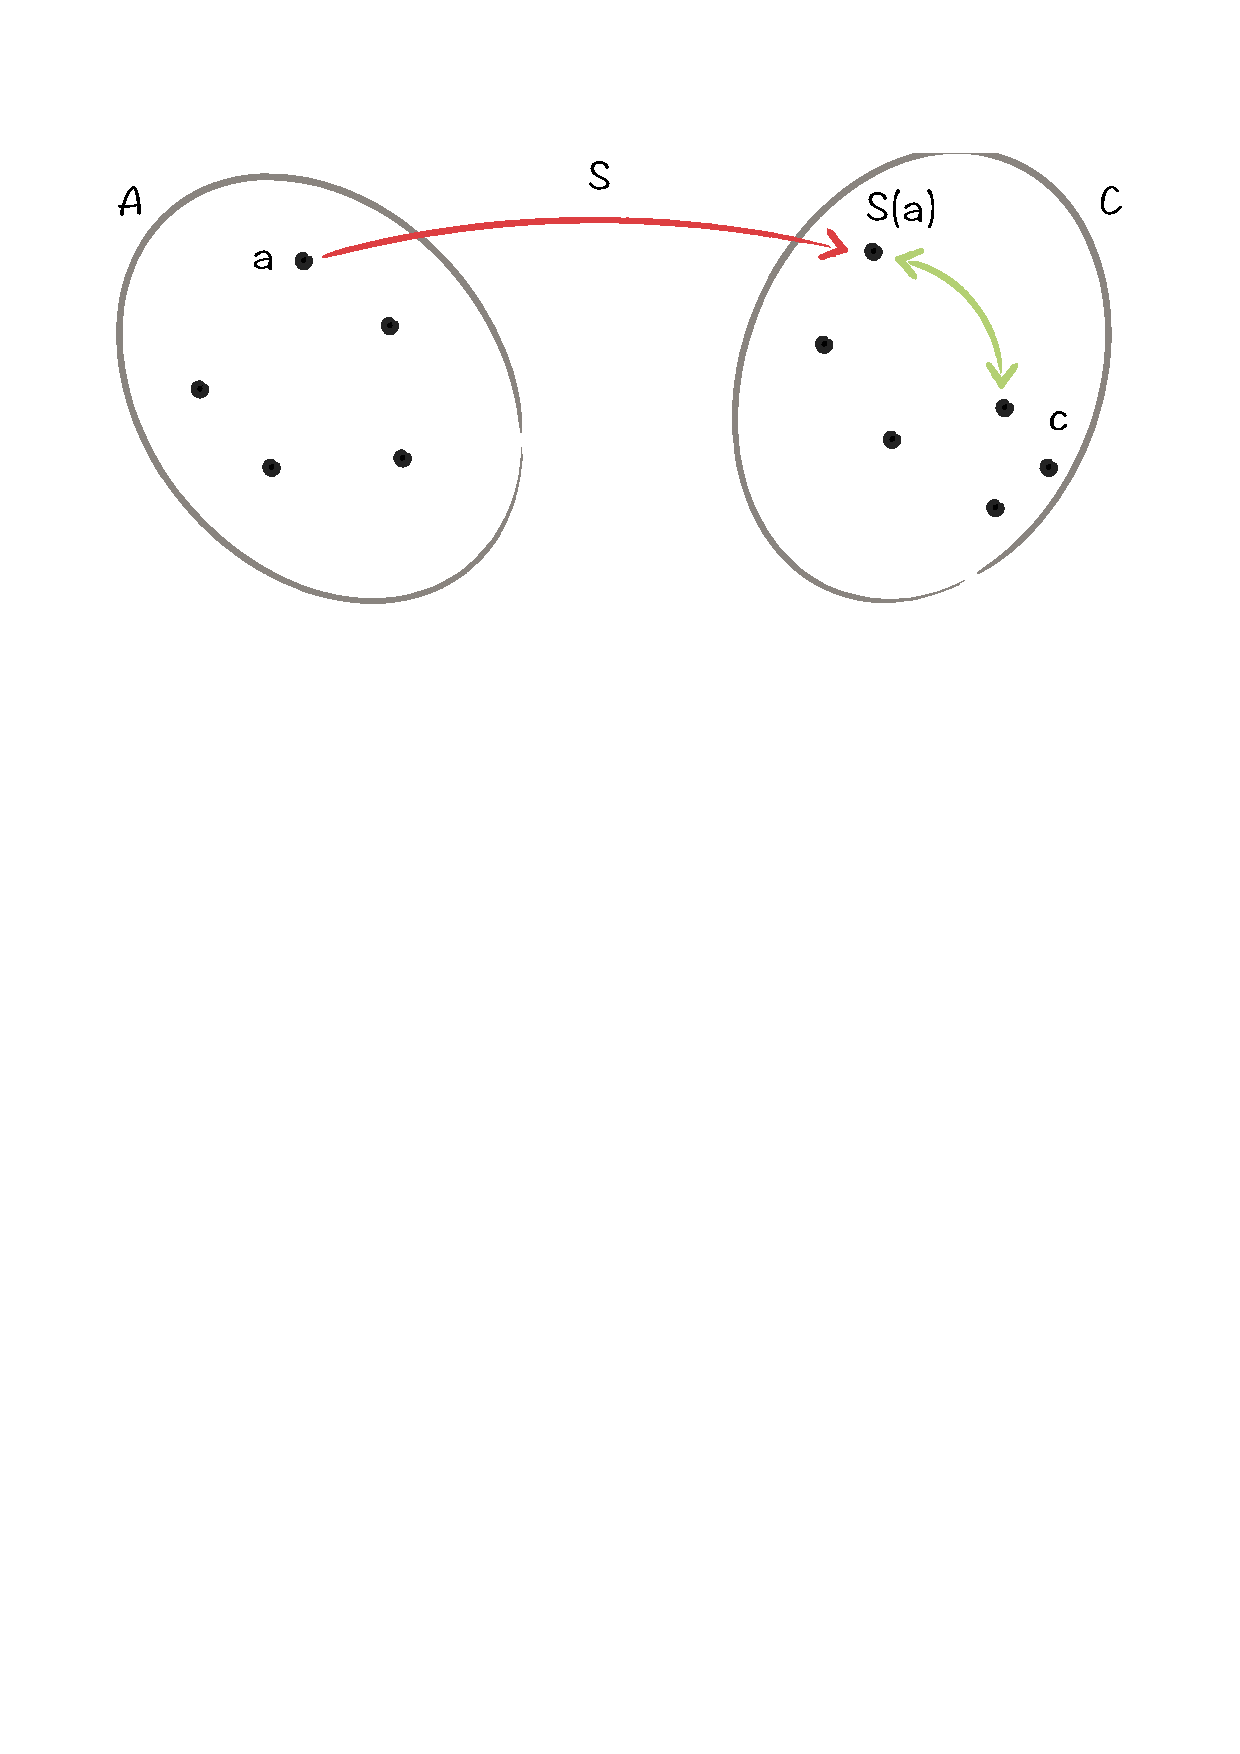
\includegraphics[width=.65\textwidth]{Figures/fig-equivalence-category.pdf}}
  \caption{Equivalence of categories.}
  \label{equivalence-category}
\end{figure}
%%###########s

\begin{Article}{Equivalence between categories, groupoids.}{}
  \label{art-Equivalence-between-categories-groupoids}
  Let $A$ and $C$ be two categories.
  Let us recall that,
  according to \cite[Chap.4\,\textsection\,4 Thm.\,1]{McL71},
  a \emph{functor}
  $$
    S \colon A \to C
  $$
  is an \emph{equivalence of categories} if and only if,
  \begin{enumerate}
    \item $S$ is full and faithful,
    \item each object $c$ in $C$ is isomorphic to $S(a)$ for some object $a$ in $A$.
  \end{enumerate}
  If $A$ and $C$ are groupoids,
  the last condition means that,
  \begin{enumerate}
    \item[(2')] for each object $c$ of $C$,
    there exists an object $a$ of $A$ and an arrow from $S(a)$ to $c$.
  \end{enumerate}
  %
  In other words:
  Let the \emph{transitivity-components} of a groupoid be the maximal full subgroupoids such that each object is connected to any other object by an arrow.
  The functor $S$ is an equivalence of groupoids if
  \begin{enumerate}
    \item it is  full and faithful,
    \item it descends surjectively on the set of transitivity-components.
  \end{enumerate}
  %
  \begin{center}
    \begin{tikzcd}[column sep=2cm, row sep=1cm,every label/.append style = {font = \small}]
      A \arrow[d, swap, "\Comp"]  \arrow[r, "S"] &  C \arrow[d,"\Comp"] \\
      \Comp(A) \arrow[r, swap, "S_*"] & \Comp(C)
    \end{tikzcd}
  \end{center}
  %
\end{Article}

\begin{Article}{Equivalence of structure-groupoids.}{}
  \label{art-Equivalence-Of-Structure-Groupoids}
  Consider an $n$-orbifold $X$.
  Let $\cA$ be an atlas,
  let $\cF$ be the associated strict generating family,
  let $\cN$ be the nebula of $\cF$ and let $\GG$ the associated structure groupoid.

  \smuline{Proposition.} {\itshape The fibers of the subduction $\Eval \colon \Obj(\GG) \to X$ are exactly the transitivity-components of $\GG$.
  In other words,
  the space of transitivity components of the groupoid $\GG$ associated with any atlas of the orbifold $X$,
  equipped with the quotient diffeology,
  is the orbifold itself.}

  %%###########
  % MARK: Figure
  %%###########
  \begin{figure}[bth]
    \centerline{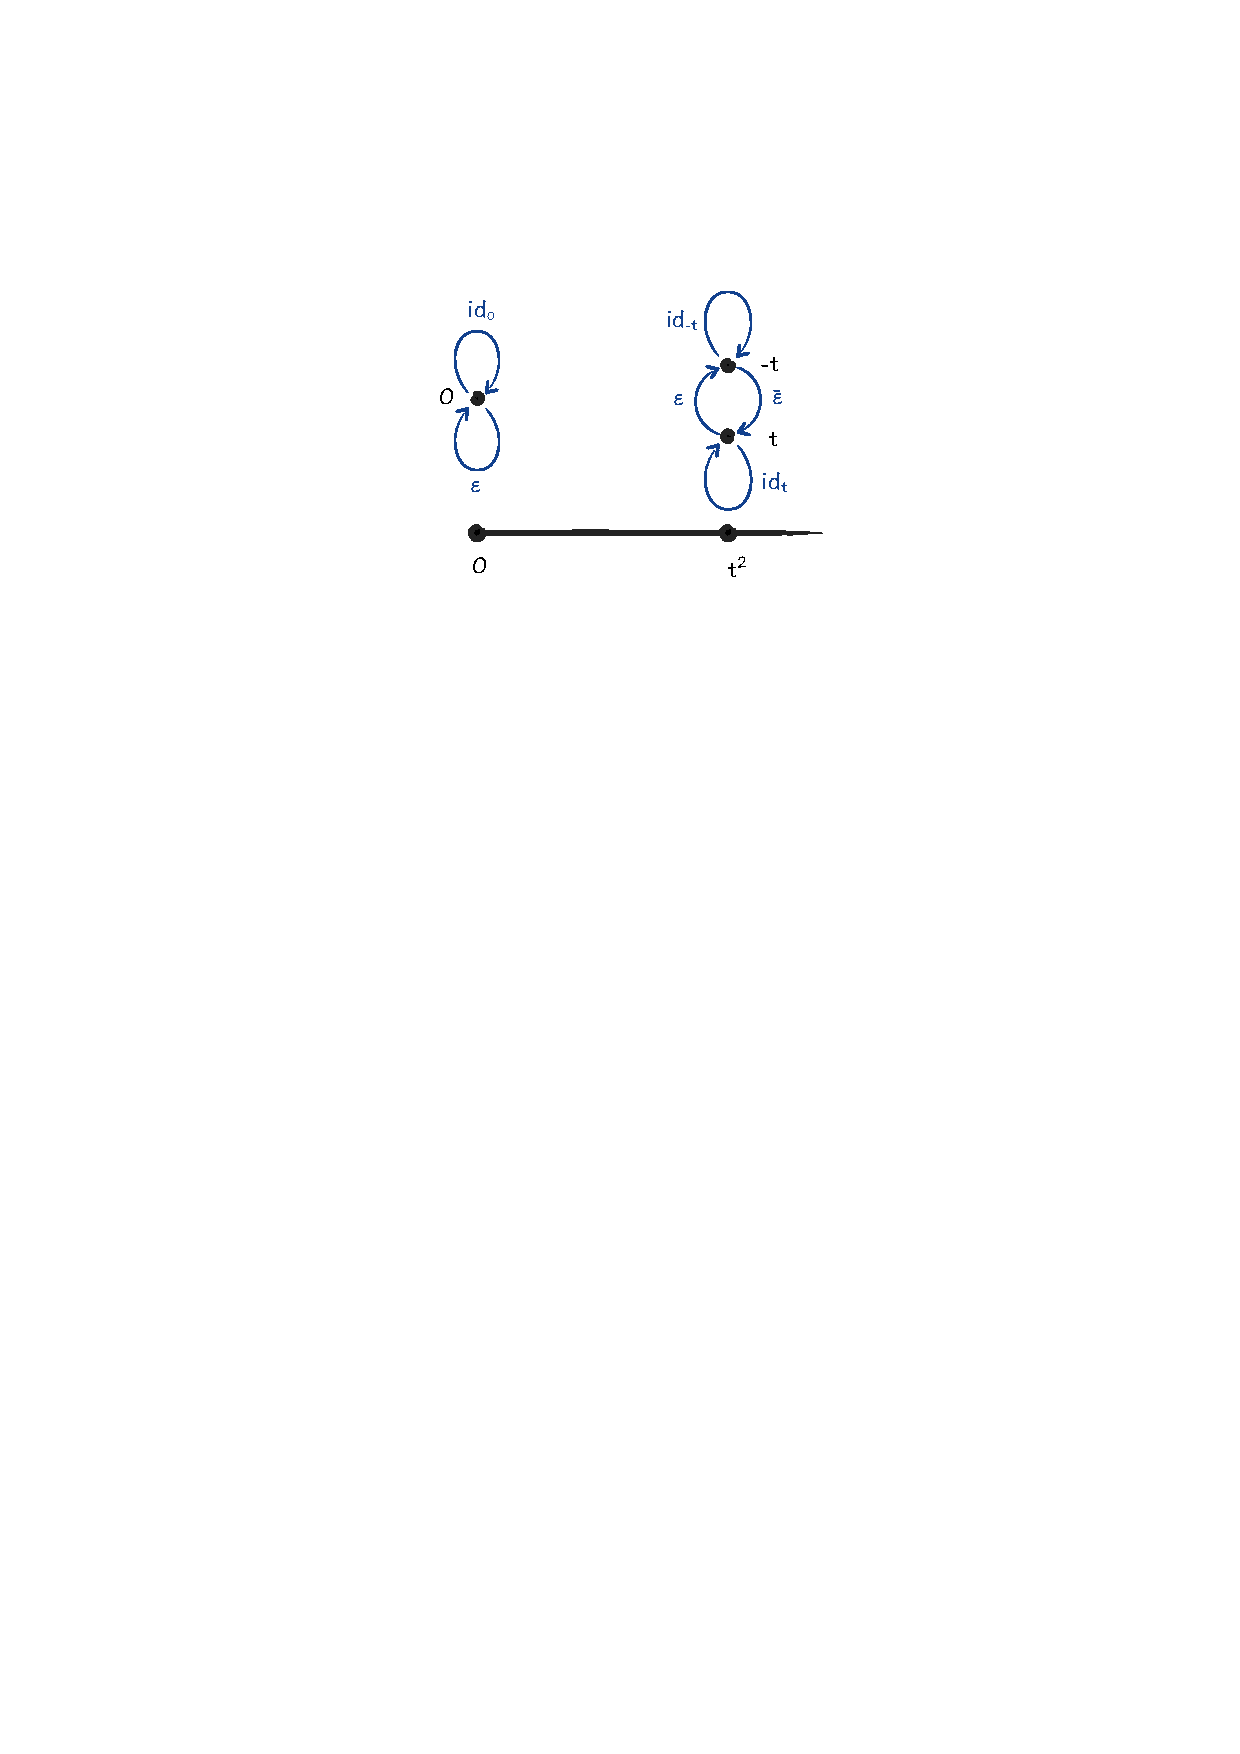
\includegraphics[width=.5\textwidth]{Figures/fig-Delta1.pdf}}
    \caption{The Groupoid of $\Delta_1$.}
    \label{fig-Delta1}
  \end{figure}
  %%###########

  \uline{Theorem.}~{\itshape Different atlases of $X$ give equivalent structure groupoids.
  The structure groupoids associated with diffeomorphic orbifold are equivalent.

  In other words,
  the equivalence class,
  in the sense of categories,
  of the structure groupoids of a orbifold is a diffeological invariant.}
\end{Article}

%%###########
% MARK: Figure
%%###########
\begin{figure}[htb]
  \centerline{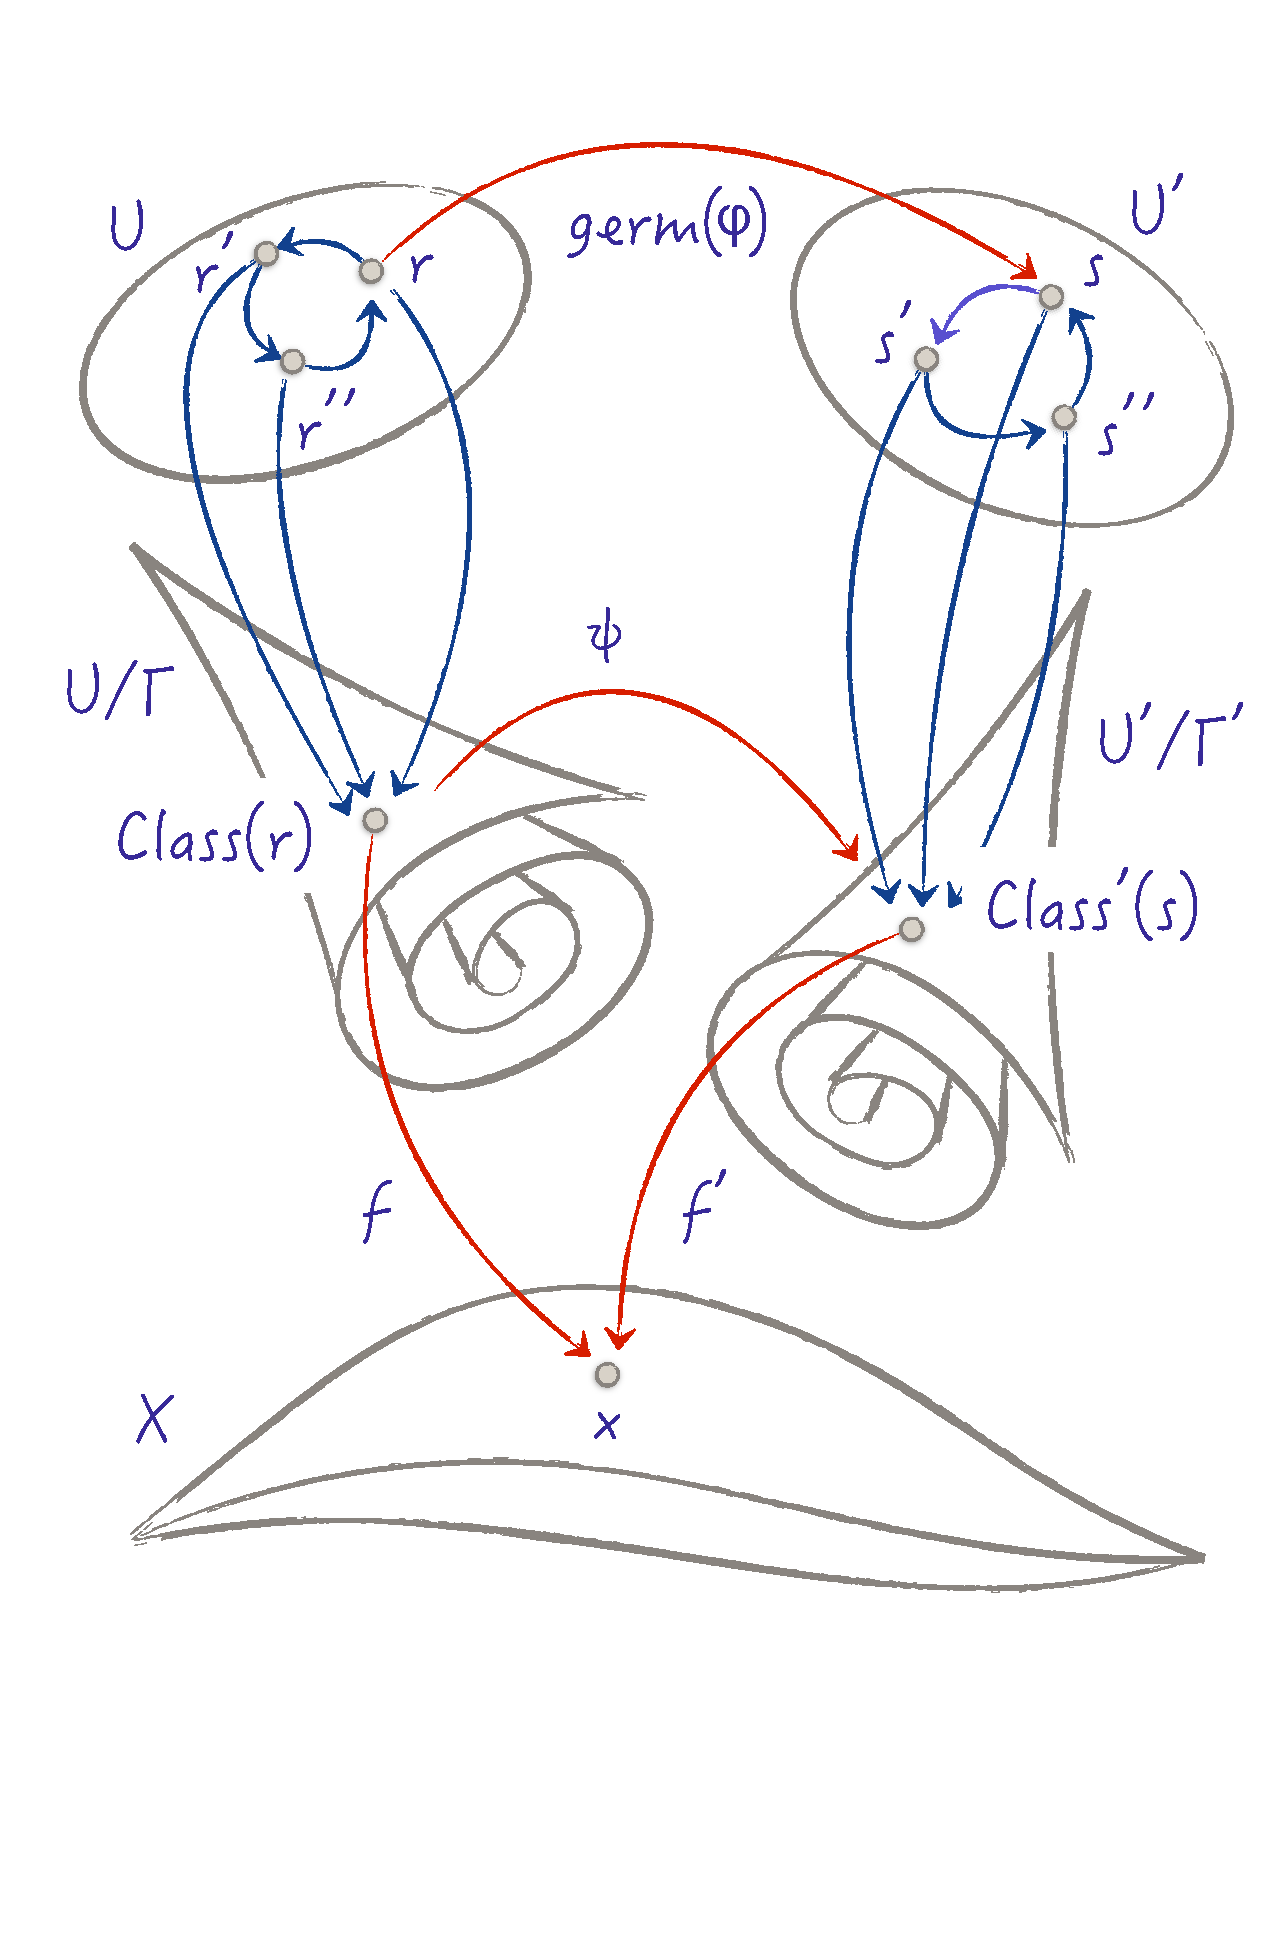
\includegraphics[width=.65\textwidth]{Figures/fig-Quasifold.pdf}}
  \caption{Lifting the identity: The Gauge Groupoid.}
  \label{fig-Quasifold}
\end{figure}
%%###########

\begin{proof}
  The proof of this theorem is based on the previous two propositions \textsection\,\ref{Lifting-The-Identity} and  \textsection\,\ref{Lifting-Local-Diffeomorphisms}.

  Let us start by proving the proposition.
  Let
  $$
    F \colon U \to X \SpacedText{and} F' \colon U' \to X'
  $$
  be two generating plots from the strict family $\cF$,
  and $r \in U \subset \RR$ and $r' \in U' \subset \RR'$.
  Assume that
  $$
    \Eval(F,r) = \Eval(F',r') = x,
    \SpacedText{that is},
    x = F(r) = F'(r').
  $$
  %
  Note that
  $$
    F = f \circ \Class \restriction U
    \SpacedText{and}
    F' = f' \circ \Class' \restriction U',
  $$
  where $f, f' \in \cA$.
  Then,
  let
  $$
    \psi = f'^{-1} \circ f
    \SpacedText{with}
    \psi \colon f^{-1}(f'(U')) \to U',
  $$
  is a local diffeomorphism that maps
  $$
    \xi = f(\Class(r))
    \SpacedText{to}
    \xi' = f'(\Class'(r')).
  $$
  Then,
  according to \textsection\,\ref{Lifting-Local-Diffeomorphisms}:

  \begin{enumerate}
    \item $n=n'$,
    \item there exists a local diffeomorphism $\varphi$ of $\RR^n$,
    lifting locally $\psi$ and  mapping $r$ to $r'$.
    That is
    $$
      \Class' \circ \pphi =_\loc \psi \circ \Class
      \SpacedText{and} \psi(r) = r'.
    $$
  \end{enumerate}
  Its germ realizes a morphism (an arrow) of the groupoid $\GG$ connecting $(F,r)$ to $(F',r')$,
  which are then on the same transitivity component:
  $$
    F(r) = F'(r') \Rightarrow \Comp(F,r) = \Comp(F',r').
  $$

  Of course,
  when $F(r) \neq F'(r')$ there cannot be an arrow, by definition.
  Therefore,
  the fibers of the evaluation map are the transitive components of the structure groupoid $\GG$ of the orbifold.

  Now,
  for the theorem:
  let $\cA$ and $\cA'$ be two atlases of $X$ and consider
  $$
    \cA'' = \cA \coprod \cA'.
  $$
  With an obvious choice of notation:
  $$
    \Obj(\GG'')=\Obj(\GG) \coprod \Obj(\GG'),
  $$
  and $\GG''$ contains naturally $\GG$ and $\GG'$ as full subgroupoids.
  The question then is:
  how does the adjunction of the crossed arrows between $\GG$ and $\GG'$ change the distribution of transitivity-components?
  According to the previous proposition,
  it changes nothing since,
  for $\GG$,
  $\GG'$ or $\GG''$,
  the set of transitivity-components are always exactly the fibers of the respective subductions $\Eval$.
  In other words,
  the set of groupoid components is always $X$,
  for any atlas of $X$.
  Thus $\GG$ and $\GG'$ are equivalent to $\GG''$,
  therefore $\GG$ and $\GG'$ are equivalent.
\end{proof}

%%%%%%%%%%%%%%%%%%%%%%%%%%%%%%%%%%%%%%%%%%%%%%%%%%%%%%%%%%
%%
%% MARK:  Quasifolds as Diffeologies
%%
%%%%%%%%%%%%%%%%%%%%%%%%%%%%%%%%%%%%%%%%%%%%%%%%%%%%%%%%%%
\section{Quasifolds as diffeologies}

The notion de \emph{quasifold} has been proposed by Elisa Prato in \cite{EP01},
it extends the notion of orbifold.
The original definition,
which has been modified once or twice,
has been revisited by diffeology as follows:

\begin{Article}{Definition.}{\it}
  \label{Quasifolds}
  A diffeological space $X$ is said to be a $n$-quasifold if it is locally diffeomorphic everywhere to a quotient $\RR^n/\Gamma$,
  where $\Gamma$ is a countable subgroup of $\Aff(\RR^n)$.

  The main difference is that the group $\Gamma$ can be infinite,
  but countable.

  \uline{Example 1.} The first example would certainly be the irrational torus $\Torus_\alpha = \RR/(\ZZ + \alpha \ZZ)$ with $\alpha \in \RR - \QQ$.
  Also quotient of the $2$-torus by the irrational solenoid $\cS_\alpha$.
  Here the subgroup is strictly affine.

  \uline{Example 2.} One can think also of the \emph{irrational cone} or \emph{quasicone}:
    $$
      \cC_\alpha = \CC/\{e^{2 i \pi k \alpha}\}_{k \in \ZZ},
    $$
    where $\alpha \in \RR - \QQ$.

    As a curiosity we have this triangle of subductions:
    \begin{center}
      \begin{tikzcd}[column sep=large, row sep=large,every label/.append style = {font = \small}]
        {} &  \CC \arrow[dl,swap, "\Class"] \arrow[dr, "\Modulus{\cdot}^2"] & {} \\
        \cC_\alpha \arrow[rr, swap, "\pi"] & {} & \Delta_2
      \end{tikzcd}
    \end{center}
    where $\Class : \CC \to \cC_\alpha$ is the standard projection from the space to its quotient,
    and $\Modulus{\cdot}^2 : z \mapsto \Modulus{z}^2$ is the projection from $\CC$ to the quotient $\CC/\U(1)$ which is equivalent to $\Delta_2 = \RR^2/\O(2)$.
    Then,
    the map $\pi : \cC_\alpha \to \Delta_2$ is a subduction since $\Class$ and $\Modulus{\cdot}^2 = \pi \circ \Class$ are both subductions \cite[\textsection\,1.51]{PIZ13}.
    The preimages of $\pi$ are all diffeomorphic to the irrational torus $\Torus_\alpha$ except for $0$.
    It would be an exercise probably to show that the local diffeomorphisms of $\cC_\alpha$ have two orbits: $\{0\}$ and $\cC_\alpha -\{0\}$.
    Note that the D-topology of $\cC_\alpha$ is certainly,
    by density,
    the pullback of the D-topology of $\Delta_2$,
    which coincides with the topology of the half-line $\LeftClosedInterval{0,\infty}$.

\end{Article}

\vfill
\centerline{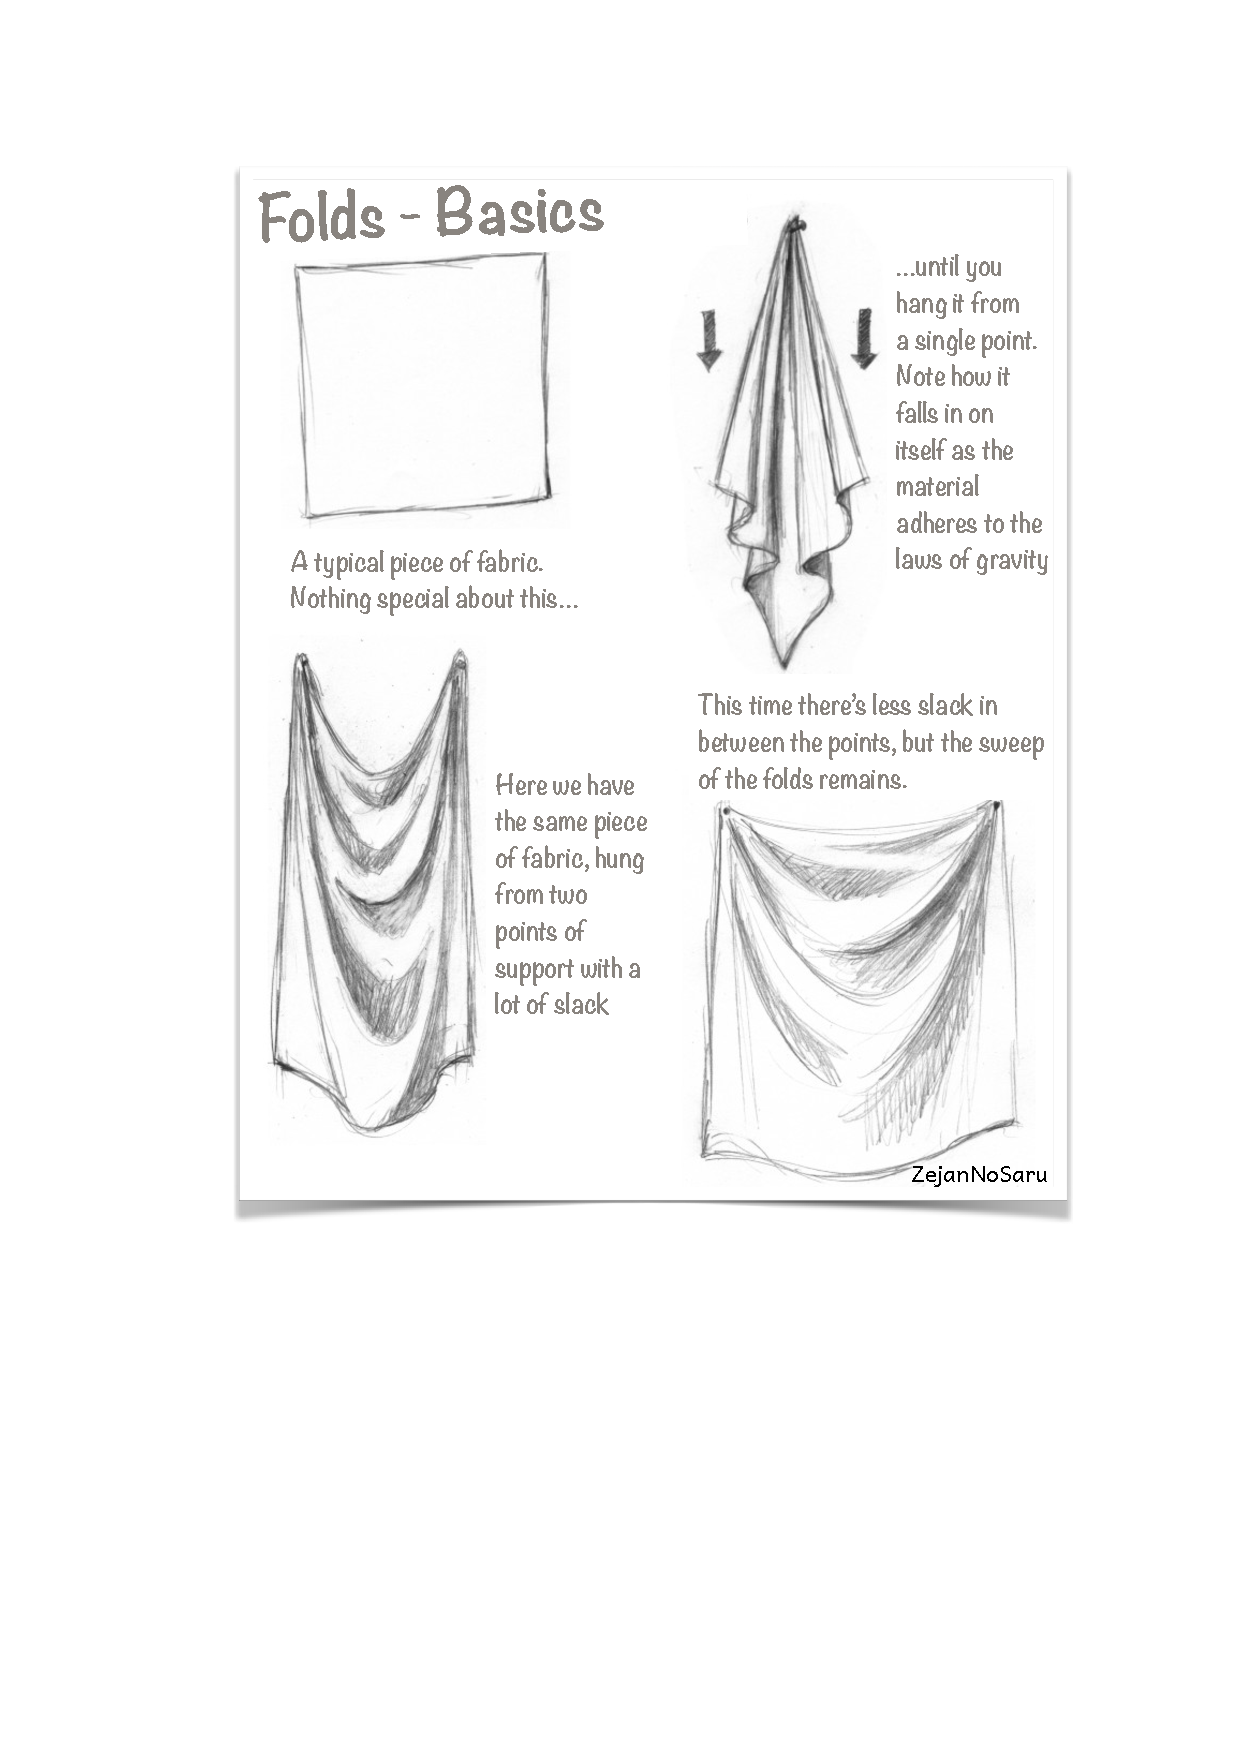
\includegraphics[width=.62\textwidth]{Figures/Folds.pdf}}
